\documentclass[12pt,UTF8]{ctexbook}
\usepackage{ctex}
\usepackage{caption}
\usepackage{graphicx}
\usepackage{float}
\usepackage{wrapfig}
\usepackage{array}
\usepackage[table, dvipsnames, svgnames, x11names]{xcolor}
\usepackage{colortbl}% 
\usepackage{tabularx}
\usepackage{amsmath}
\usepackage{amssymb}
\usepackage{xfrac}
\usepackage{eucal}
\usepackage{titlesec}
\usepackage{amsthm}
\usepackage{tikz-cd}
\usepackage{enumitem}
\usepackage{verbatim}
\usepackage{fontspec,xunicode,xltxtra}
\usepackage{xeCJK} 

\definecolor{gl}{RGB}{246, 252, 240}
\definecolor{gd}{RGB}{236, 244, 230}
\definecolor{bg}{RGB}{242, 244, 228}


\setCJKmainfont[BoldFont=STZhongsong]{STSong}
\setCJKmonofont{simkai.ttf} % for \texttt
\setCJKsansfont{simfang.ttf} % for \textsf
\setlength\parskip{8pt}
\setlength{\fboxsep}{12pt}
\renewcommand\thesection{\arabic{chapter}.\arabic{section}}
\newtheorem{df}{定义}[section] 
\newtheorem{pp}{命题}[section]
\newtheorem{tm}{定理}[section]
\newtheorem{ex}{例子}[section]
\newtheorem{sk}{思考}[section]
\newtheorem{po}{公理}
\newtheorem*{so}{解答}
\newenvironment{proof2}{\paragraph{\textbf{证明:}}}{\hfill$\square$}
\newtheorem{xt}{习题}[section]
\newtheorem{cor}{推论}[pp]
% 列举环境的行间距
\setenumerate[1]{itemsep=0pt,partopsep=0pt,parsep=0pt,topsep=0pt}
\setitemize[1]{itemsep=0pt,partopsep=0pt,parsep=0pt,topsep=0pt}
\setdescription{itemsep=0pt,partopsep=0pt,parsep=0pt,topsep=0pt}
\setlength{\intextsep}{2pt}%
\setlength{\columnsep}{2pt}%
% 新函数
\renewcommand\parallel{\mathrel{/\mskip-4mu/}}
% 章节字体大小
\titleformat{\section}{\zihao{-2}\bfseries}{ \thesection }{16pt}{}
% 封面
\title{\zihao{0} \bfseries 第三册}
\author{\zihao{2} \texttt{大青花鱼}}
% \date{\bfseries\today}
\date{}
% 正文
\begin{document}
\maketitle
\tableofcontents
\newpage

\chapter{相似三角形}
形状一样,大小不同,我们把这样的关系称为相似关系。三角形之间自然也存在相似关系。
如果两个三角形对应的内角都相等或都相反,就说它们\textbf{同角相似}或\textbf{反角相似},统称\textbf{相似}。
一般用$\sim$和$\backsim$表示两个三角形同角和反角相似。如果不要求区分,可以只用$\sim$表示相似。

\begin{wrapfigure}{r}{0.26\textwidth} %this figure will be at the right
    \vspace{-26pt}
    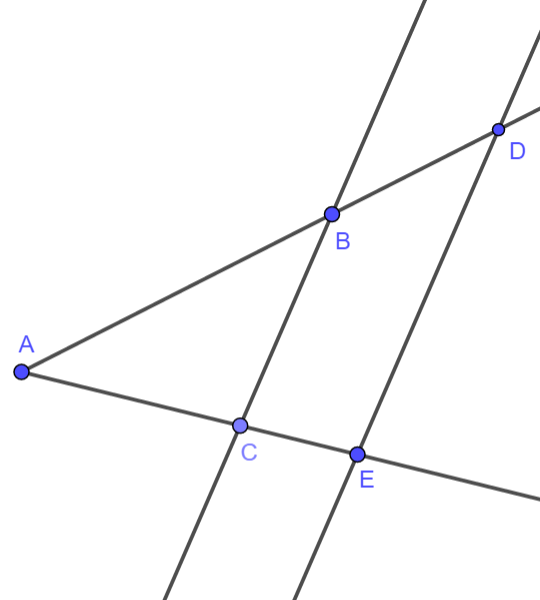
\includegraphics[width=0.26\textwidth]{比例1.png}
\end{wrapfigure}

相似关系比全等关系的要求宽松一些。只要两个三角形全等,它们必然相似。反之,两个三角形相似,它们未必全等。

\section{平行与相似}
我们已经学习过相似关系的基本公理:
\begin{po}{\textbf{放缩公理}}\label{po:6}
    从一点$A$出发的两条射线,每条线上取两点:$B,D$和$C,E$。如果
    $$ \frac{|AB|}{|AD|} = \frac{|AC|}{|AE|},$$
    那么,
    $$ \frac{|AB|}{|AD|} = \frac{|AC|}{|AE|} = \frac{|BC|}{|DE|},$$
    而且$\angle ABC = \angle ADE$,$\angle ACB = \angle AED$。
\end{po}

放缩公理说明,从一点出发的两条射线被两条直线所截,如果截得的线段成相同的比例,那么这两条直线平行。
注意到两条平行线截出了两个三角形:$\triangle ABC$和$\triangle ADE$,它们的三个内角分别相等。
所以$\triangle ABC$和$\triangle ADE$相似。我们把$\frac{|AB|}{|AD|}$称为两者的\textbf{相似比}。

% \begin{wrapfigure}{r}{0.28\textwidth} %this figure will be at the right
%     \vspace{-10pt}
%     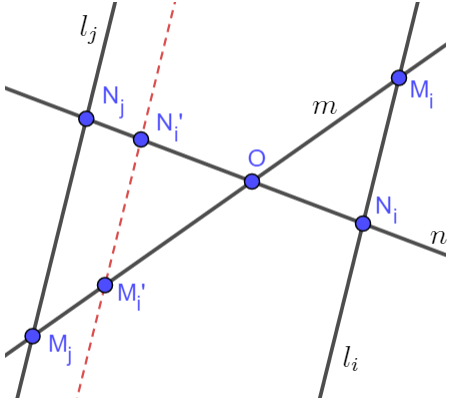
\includegraphics[width=0.28\textwidth]{相似2.png}
% \end{wrapfigure}

反之,通过平行公理可以推出,如果从一点出发的两条射线被两条平行直线所截,那么截得的线段成相同的比例,截得的三角形相似。
甚至,“射线”可以改为“直线”。
% TODO 补上证明

一般来说,如果两个三角形相似,它们对应的边是否成比例呢?
\begin{tm}\label{tm:0-0-1}
    三角形相似,则相等内角的对边成比例。
\end{tm}
\begin{proof2}
    设有三角形:$\triangle ABC \sim \triangle A'B'C'$,即$\angle BAC = \angle B'A'C'$,
    $\angle CBA = \angle C'B'A'$,$\angle BCA = \angle B'C'A'$。在射线$AB$上找一点$D$,使得$|AD| = |A'B'|$,
    在射线$AC$上找一点$E$,使得$|AE| = |A'C'|$。根据“边角边”,$\triangle ADE \simeq \triangle A'B'C'$。
    于是,$\angle DEA = \angle B'C'A' = \angle BCA$。同位角相等,即$DE \parallel BC$。因此
    $$ \frac{|AB|}{|AD|} = \frac{|AC|}{|AE|} = \frac{|BC|}{|DE|}.$$
    即
    $$ \frac{|AB|}{|A'B'|} = \frac{|AC|}{|A'C'|} = \frac{|BC|}{|B'C'|}.$$
    如果$\triangle ABC \backsim \triangle A'B'C'$,同样方法作出的$\triangle ADE \backsimeq \triangle A'B'C'$。
    于是通过类似推理可以得到相同的结论。
\end{proof2}

\section{判定相似关系}
如何判断两个三角形是否相似呢?方法和判断三角形是否全等差不多。

\begin{tm}\label{tm:0-1-0}
    给定$\triangle ABC$和$\triangle A'B'C'$。如果$\angle BAC = \angle B'A'C'$或$\angle BAC = \angle C'A'B'$成立,
    且
    $$ \frac{|AB|}{|A'B'|} = \frac{|AC|}{|A'C'|},$$
    那么$\triangle ABC$和$\triangle A'B'C'$相似。
\end{tm}
这显然是放缩公理的直接应用。
在射线$AB$、$AC$上分别找到点$D$和$E$,使得$|AD| = |A'B'|$,
$|AE| = |A'C'|$,根据“边角边”,$\triangle ADE \cong \triangle A'B'C'$。
于是根据放缩公理,$\triangle ABC$和$\triangle ADE$相似,故而和$\triangle A'B'C'$相似。
我们把这个判断方法也简称为“边角边”。
和全等三角形“边角边”一样,$\angle BAC = \angle B'A'C'$和$\angle BAC = \angle C'A'B'$的情况分别对应同角和反角相似。

判定全等的“角边角”则化为显然的结论:如果两个三角形有两个内角分别相等,则它们相似。

最后,“边边边”则对应定理\ref{tm:0-0-1}的逆命题:
\begin{tm}\label{tm:0-1-1}
    三角形对应的三边成比例,则它们相似。
\end{tm}
\begin{proof2}
    设$\triangle ABC$和$\triangle A'B'C'$满足:
    $$ \frac{|AB|}{|A'B'|} = \frac{|AC|}{|A'C'|} = \frac{|BC|}{|B'C'|}.$$
    在在射线$AB$上找一点$D$,使得$|AD| = |A'B'|$,
    在射线$AC$上找一点$E$,使得$|AE| = |A'C'|$。则
    $$ \frac{|AB|}{|AD|} = \frac{|AB|}{|A'B'|} = \frac{|AC|}{|A'C'|} = \frac{|AC|}{|AE|},$$
    根据放缩公理,
    $$ \frac{|AB|}{|AD|} = \frac{|AC|}{|AE|} = \frac{|BC|}{|DE|},$$
    这说明
    $$ |DE| = \frac{|BC|\cdot |AD|}{|AB|} = \frac{|BC|\cdot |A'B'|}{|AB|} = |B'C'|. $$
    根据“边边边”,$\triangle ADE \cong \triangle A'B'C'$。因此$\triangle ABC \sim \triangle A'B'C'$。
\end{proof2}

我们把这个结论也简称为“边边边”。和判定三角形全等的“边边边”一样,我们无法确定是同角相似还是反角相似。

\section{相似三角形性质与应用}

\begin{wrapfigure}{r}{0.27\textwidth} %this figure will be at the right
    \vspace{-10pt}
    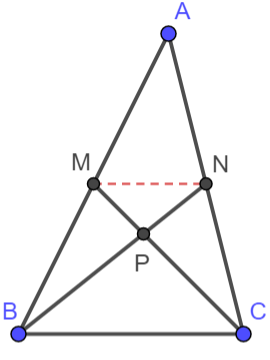
\includegraphics[width=0.27\textwidth]{三角形8.png}
\end{wrapfigure}

相似三角形性质在研究一般三角形性质的时候很有用,因为,我们接下来会看到,三角形里面有很多有趣的相似现象。

\begin{tm}\label{tm:0-2-0}
    三角形顶点和对边中点确定的直线称为该边的中线。设$\triangle ABC$的边$AB$中点为$M$,
    边$AC$的中点为$N$,过$M$的中线$CM$和过$N$的中线$BN$交于一点$P$,则
    $$\frac{|BP|}{|PN|} = \frac{|CP|}{|PM|} = 2.$$
\end{tm}
\begin{proof2}
    从已知条件可以得到:
    $$\frac{|AM|}{|AB|} = \frac{|AN|}{|AC|} = \frac12.$$
    因此,作辅助线$MN$。根据放缩公理,$\triangle AMN \sim \triangle ABC$,相似比为$\frac12$。
    即$|BC| = 2|MN|$。此外还推出$MN \parallel BC$,因此,$\triangle PMN \sim \triangle PCB$。因而有
    $$\frac{|BP|}{|PN|} = \frac{|CP|}{|PM|} = \frac{|BC|}{|MN|} = 2.$$
\end{proof2}

\begin{wrapfigure}{r}{0.27\textwidth} %this figure will be at the right
    \vspace{-10pt}
    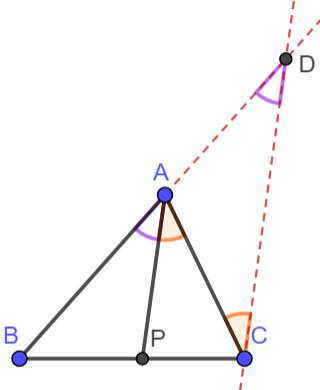
\includegraphics[width=0.27\textwidth]{三角形9.png}
\end{wrapfigure}

$MN$也叫做关于边$BC$的中位线。另外要注意的是:我们只知道点$P$把中线分成长度$2:1$的两段,
并不知道中线本身有多长。

\begin{tm}\label{tm:0-2-1}
    设三角形$\triangle ABC$的内角$\angle BAC$的角平分线交对边于$P$,则
    $$ \frac{|BP|}{|PC|} = \frac{|BA|}{|AC|}.$$
\end{tm}
\begin{proof2}
    过$C$作$AP$的平行线,与射线$BA$交于点$D$。$CD \parallel AP$,所以同位角$\angle BAP = \angle BDC$,
    内错角$\angle PAC = \angle DAC$。而$AP$是角平分线,所以$\angle BAP = \angle PAC$。
    于是$\angle BDC = \angle DAC$,$\triangle ACD$是等腰三角形,$|AC| = |AD|$。\\
    另一方面,$CD \parallel AP$,所以$\triangle BAP \sim \triangle BDC$,因此,
    $$\frac{|BP|}{|PC|} = \frac{|BA|}{|AD|} = \frac{|BA|}{|AC|}.$$
\end{proof2}

\begin{wrapfigure}{r}{0.27\textwidth} %this figure will be at the right
    \vspace{-80pt}
    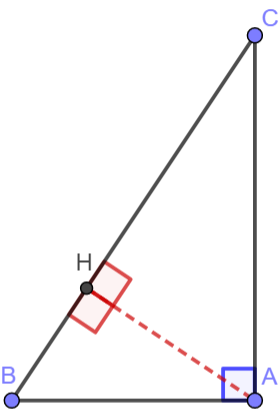
\includegraphics[width=0.27\textwidth]{三角形10.png}
\end{wrapfigure}

我们利用角平分线的性质构造了一个等腰三角形。这是与角平分线相关的问题中常见的思路。
相应地,也可以过$B$作$AC$的平分线,和$AP$交于点$E$,并证明$\triangle ABE$是等腰三角形。

\begin{tm}{\textbf{射影定理}}\label{tm:0-2-2}
    直角三角形$ABC$中,$\angle A$是直角。作$A$到$BC$的垂线,垂足为$H$。则
    $$ |AB|^2 = |BH|\cdot |BC|, \quad |AC|^2 = |CH|\cdot |BC|,$$
    且
    $$|AH|^2 = |BH| \cdot |CH|.$$
\end{tm}
\begin{proof2}
    $\angle AHB$和$\angle BAC$都是直角。
    $\angle HBA = \angle CBA$,$\angle AHB = \angle BAC$,所以$\triangle HBA \sim \triangle ABC$。
    因此,
    $$ \frac{|BH|}{|BA|} = \frac{|BA|}{|BC|},$$
    即
    $$ |AB|^2 = |BH|\cdot |BC|.$$
    同理,
    $\angle ACH = \angle ACB$,$\angle CHA = \angle BAC$,所以$\triangle HAC \sim \triangle ABC$。
    因此,
    $$ \frac{|CH|}{|AC|} = \frac{|CA|}{|BC|},$$
    即
    $$ |AC|^2 = |CH|\cdot |BC|.$$
    从$\triangle HBA \sim \triangle ABC$可以推出$\angle BAH = \angle ACB$,
    从$\triangle HAC \sim \triangle ABC$可以推出$\angle HAC = \angle CBA$,
    因此,$\triangle HAC \sim \triangle HBA$。于是,
    $$ \frac{|BH|}{|HA|} = \frac{|AH|}{|HC|},$$
    即
    $$|AH|^2 = |BH| \cdot |CH|.$$
\end{proof2}

射影定理是一个十分有用的结论。
它的本质是直角三角形中的相似关系:$\triangle HAC \sim \triangle HBA \sim \triangle ABC$。

\begin{tm}{\textbf{勾股定理}}\label{tm:0-2-3}
    直角三角形$ABC$中,$\angle A$是直角。则
    $$|AB|^2+|AC|^2 = |BC|^2.$$
\end{tm}
\begin{proof2}
    作$A$到$BC$的垂线,垂足为$H$。
    根据射影定理,    
    $$ |AB|^2 = |BH|\cdot |BC|, \quad |AC|^2 = |CH|\cdot |BC|,$$
    这说明
    $$ |AB|^2+|AC|^2 = |BH|\cdot |BC| + |HC|\cdot |BC| = (|BH| + |HC|)\cdot |BC|$$
    即
    $$ |BC|^2 = |AB|^2+|AC|^2.$$
\end{proof2}

勾股定理是数学中非常重要的定理,也是非常有名的定理。它的证明方法有四百多种,涉及各种各样的技巧和知识。
勾股定理在西方也称为毕达哥拉斯定理。

从勾股定理出发,可以得出这样的推论:
\begin{cor}{\textbf{垂距定理}}\label{cr:0-2-0}
    记直线$l$外一点$P$到直线$l$的垂足为$D_P$,那么$P$到$l$上任一点$Q$的距离,不小于它到$D_P$的距离。
    $$ |PQ | \geqslant |PD_P|.$$
    如果$Q \neq D_P$,那么$|PQ| > |PD_P|$。
\end{cor}

\begin{df}{\textbf{点到直线的距离}}\label{df:0-2-0}
    一点$P$到直线$l$的距离,就是它到$l$上所有点距离的最小值。
\end{df}
根据垂距定理,记$P$到直线$l$的垂足为$D_P$,那么点$P$到$l$的距离就是$|PD_P|$。

\begin{sk}\label{sk:0-2-0}
    能不能定义一条直线到另一条直线的距离?如果能,怎么定义?如果不能,为什么?
\end{sk}

\begin{xt}\label{xt:0-2-0} 证明垂距定理。
\end{xt}


\chapter{三角形的四线五心}
证明三角形性质的时候,我们用到了三角形的中点和辅助线。三角形的特殊点和相关辅助线对我们了解三角形的性质是很有帮助的。
接下来我们会介绍四种常见的特殊点和相应的辅助线。它们一般合称为三角形的四线。

\section{垂直平分线和外心}
垂直平分线定理告诉我们,三角形每条边都对应一条称为垂直平分线的直线。这条直线是到它的两个端点距离相等的点的集合,
是过它的中点,且与它垂直的直线。三角形的三边,对应三条垂直平分线。这三条垂直平分线有什么联系呢?

我们先看两条垂直平分线的关系。给定三角形$ABC$,记顶点$A$对边的垂直平分线为$p(A)$,$B$对边的垂直平分线为$p(B)$。
按照定义,$p(A)$垂直于直线$BC$,$p(B)$垂直于直线$AC$。如果$p(A)$和$p(B)$相交于点$O$,那么因为$O$在$p(A)$上,$|OB| = |OB|$;
同理,也有$|OA| = |OC|$。于是$|OA| = |OB|$,$O$也在$C$对边的垂直平分线$p(C)$上。
也就是说,三角形三边的垂直平分线都交于点$O$。

那么,$p(A)$和$p(B)$是否总相交呢?两条直线要么相交,要么平行或重合。
如果$p(A)$和$p(B)$平行或重合,根据垂直定理及推论,直线$BC$和$AC$平行或重合。
因此,要么$A,B,C$共线,这时我们说三角形退化为直线;要么$p(A)$和$p(B)$相交。
\begin{tm}{\textbf{外心定理}}\label{tm:1-0-0}
    (非退化的)三角形三边的垂直平分线交于一点,称为三角形的\textbf{外心}。
\end{tm}
按照定义,外心到三角形三个顶点的距离相同。

\section{垂线和垂心}

\begin{wrapfigure}[6]{r}{0.45\textwidth} %this figure will be at the right
    \vspace{-45pt}
    \flushright
    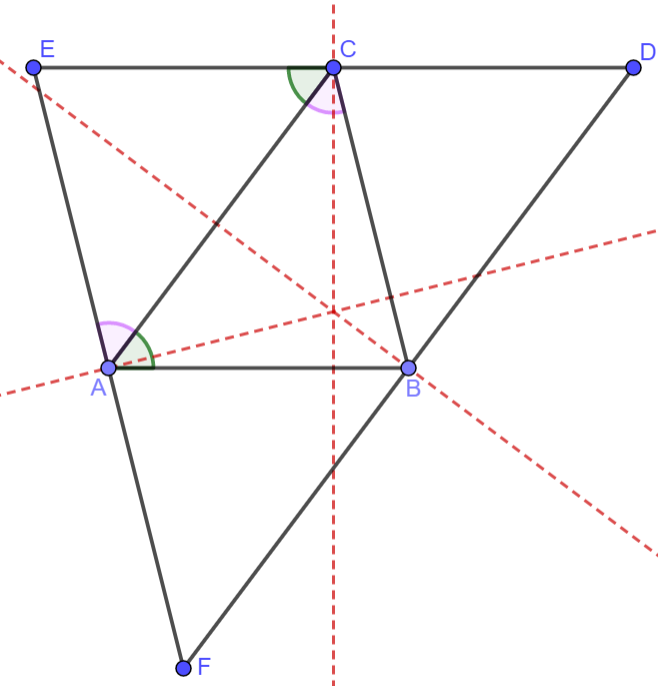
\includegraphics[width=0.4\textwidth]{三角形7.png}
\end{wrapfigure}

垂线定理告诉我们,过三角形每个顶点,都有唯一垂直于对边的直线。
我们把$A$到对边$BC$的垂线记为$h(A)$,$B$到$CA$的垂线记为$h(B)$,$C$到$AB$的垂线记为$h(C)$。
它们也叫三角形的\textbf{高线}。对应的垂足记为$H_A$、$H_B$、$H_C$。
这三条直线有什么关系呢?

\begin{tm}{\textbf{垂心定理}}\label{tm:1-1-0}
    (非退化的)三角形三边的垂线交于一点,称为三角形的\textbf{垂心}。
\end{tm}

\begin{proof2}
    如右图,过三角形顶点$A,B,C$分别作平行于对边的直线,它们两两相交于$D,E,F$。
    $\angle BAC$和$\angle ECA$是内错角,所以相等。同理,$\angle ACB = \angle CAE$。
    此外$|AC| = |CA|$。因此,根据“角边角”,$\triangle ABC \cong \triangle CEA$。
    于是$|CE| = |AB|$,$|AE| = |BC|$。\\
    类似地,有$\triangle ABC \cong \triangle DCB$,$\triangle ABC \cong \triangle BAF$。
    因此,$|CD| = |AB|$,$|BD| = |AC|$,$|BF| = |AC|$,$|AF| = |BC|$。进而可得,
    $A$是线段$EF$中点,$B$是线段$DF$中点,$C$是线段$DE$中点。垂线$h(A), h(B), h(C)$分别是
    三角形$DEF$三边的垂直平分线。根据外心定理\ref{tm:1-0-0},它们交于一点。
\end{proof2}
\begin{xt}\label{xt:1-1-0}
    \mbox{}\\
    给定三角形$ABC$的垂心$H$,\\
    1. 证明:$B$是三角形$ACH$的垂心。\\
    2. $A,B,C,H$四点之间有什么关系?\\
    过锐角三角形$ABC$的顶点$A$作$BC$的垂线,交$BC$于点$H_A$。\\
    1. 请用$|AH_A|$、$|BC|$和$|H_AC|$表示$|AC|$和$|AB|$。\\
    2. $|AC|^2$和$|AB|^2 + |BC|^2$有什么关系?\\
    3. 如果$\triangle ABC$是钝角三角形,$\angle C$是钝角,你能得到什么结论?\\
    4. 请写出勾股定理的逆命题。它是否成立?
\end{xt}

\section{角平分线、内心和旁心}

\begin{wrapfigure}{r}{0.32\textwidth} %this figure will be at the right
    \vspace{-40pt}
    \flushright
    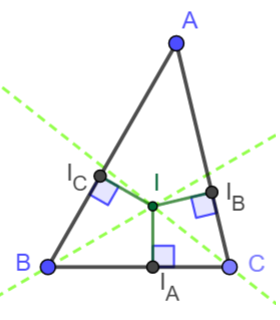
\includegraphics[width=0.28\textwidth]{三角形内心.png}
\end{wrapfigure}

三角形每个内角和外角都有角平分线,分别叫内角平分线和外角平分线。

\begin{tm}{\textbf{内心定理}}\label{tm:1-2-0}
    (非退化的)三角形内角的平分\\
    线交于一点,称为三角形的\textbf{内心}。
\end{tm}

\begin{proof2}
    设$\triangle ABC$的内角:$\angle B$和$\angle C$的平分线交于一点$I$,
    作$I$到三角形三边的垂线,设垂足分别为$I_A$、$I_B$、$Q_C$。
    根据角平分线定理,$|I_AI| = |I_BI|$、$|I_AI| = |I_CI|$。所以$|I_CI| = |I_BI|$,
    根据角平分线定理的逆定理,$I$也在$\angle A$的平分线上。
\end{proof2}

\begin{wrapfigure}{r}{0.32\textwidth} %this figure will be at the right
    \vspace{-30pt}
    \flushright
    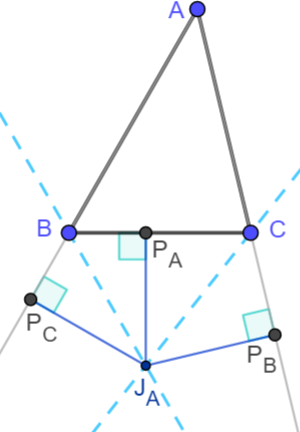
\includegraphics[width=0.28\textwidth]{三角形旁心.png}
\end{wrapfigure}

三角形的内心可以看作到三边距离相等的点。作为对比,外心是到三个顶点距离相等的点。
三角形的内角平分线和外角平分线也有交点。在以上证明的启发下,我们自然也猜测外角平分线有类似的“心”。

\begin{tm}{\textbf{旁心定理 }}\label{tm:1-2-1}
    (非退化的)三角形任一内\\
    角的平分线和另外两个外角的平分线交于一点,称为三
    角形的\textbf{旁心}。
\end{tm}

\begin{proof2}
    设$\triangle ABC$的外角:$\angle B$和$\angle C$的平分线交于一点$J_A$,
    作$J_A$到三角形三边所在直线的垂线,设垂足分别为$P_A$、$P_B$、$P_C$。
    根据角平分线定理,$|P_AJ_A| = |P_BJ_A|$、$|P_AJ_A| = |P_CJ_A|$。所以$|P_CJ_A| = |P_BJ_A|$,
    根据角平分线定理的逆定理,$J_A$也在内角$\angle A$的平分线上。
\end{proof2}

三角形每个内角和另外两个外角都可以构造一个旁心,所以,三角形有一个内心和三个旁心。

如果我们把三个旁心连成三角形,就会发现,原三角形的顶点在新三角形的边上,
而且恰好是新三角形顶点到对边的高线的垂足。我们把这个新三角形称为原三角形的\textbf{旁心三角形}。

原三角形的内角平分线就是旁心三角形的高线,所以内心作为原三角形内角平分线的交点,
就是旁心三角形的垂心。

\begin{figure}[h] %this figure will be at the right
    \centering
    \vspace{10pt}
    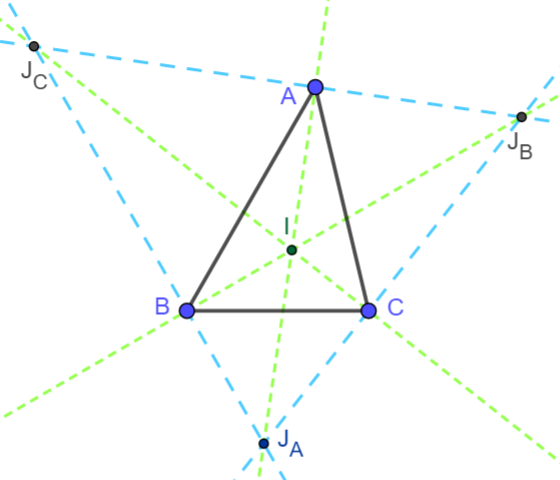
\includegraphics[width=0.5\textwidth]{三角形内心旁心.png}
\end{figure}

\begin{xt}\label{xt:1-2-0}
    \mbox{}\\
    给定三角形$ABC$的内心$I$和旁心$J_A$、$J_B$、$J_C$,证明:\\
    1. $A$在$J_BJ_C$上,$B$在$J_AJ_C$上,$C$在$J_AJ_B$上。\\
    2. $AJ_A \perp J_BJ_C$,$BJ_B \perp J_AJ_C$,$CJ_C \perp J_AJ_B$。\\
    3. $I$是三角形$J_AJ_BJ_C$的垂心。
    % 给定三角形$ABC$的高线$AH_A$、$BH_B$、$CH_C$和垂心$H$,证明:\\
    % 1. $\angle H_BH_AA = \angle AH_AH_C$。\\
    % 2. $H$是三角形$H_AH_BH_C$的内心。
\end{xt}

\section{中线和重心}
\begin{wrapfigure}{r}{0.27\textwidth} %this figure will be at the right
    \vspace{-60pt}
    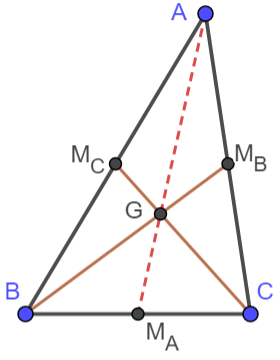
\includegraphics[width=0.27\textwidth]{三角形重心证明.png}
\end{wrapfigure}
三角形每个顶点和对边中点的连线,称为这个顶点到对边的\textbf{中线}或该边上的中线。我们已经学习过
等腰三角形和直角三角形中线的性质。等腰三角形的三条中线交于一点。一般情况下,这件事也成立。

\begin{tm}{\textbf{重心定理}}\label{tm:1-3-0}
    (非退化的)三角形三边上的中
    线交于一点,称为三角形的\textbf{重心}。
\end{tm}
\begin{proof2}
    设$\triangle ABC$三边中点为$M_A$、$M_B$、$M_C$,中线$BM_B$和$CM_C$交于点$G$。
    根据定理\ref{tm:0-2-0},
    $$\frac{|BG|}{|GM_B|} = \frac{|CG|}{|GM_C|} = 2.$$
    也就是说,$G$在线段$BM_B$上,而且$|BG| = \frac23 |BM_B|$。同理,设中线$BM_B$和$AM_A$交于点$G'$。也有:
    $$\frac{|BG|}{|G'M_B|} = \frac{|AG'|}{|G'M_A|} = 2.$$
    $G$和$G'$都在线段$BM_B$上,且$|BG| = \frac23 |BM_B| = |BG'|$。
    这说明$G$和$G'$是同一点,它是$AM_A$、$BM_B$和$CM_C$的公共点。
\end{proof2}
三角形的三条中线不仅交于一点,而且这一点到每个定点的距离,都是到对边中点距离的两倍。

重心的概念有物理的意义。均匀分布的物体受到的重力,可以视为重心受到的重力。
\begin{xt}\label{xt:1-3-0}
    $\triangle ABC$的中线$AM_A$、$BM_B$和$CM_C$交于重心$G$,讨论:\\
    1. $\triangle BGC$的面积和$\triangle ABC$的面积有什么关系?$\triangle BGA$和$\triangle AGC$呢?\\
    2. $\triangle AM_BM_C$的面积和$\triangle ABC$的面积有什么关系?$\triangle BM_AM_C$和$\triangle CM_AM_B$呢?\\
    3. $\triangle GM_BM_C$的面积和$\triangle ABC$的面积有什么关系?$\triangle GM_AM_C$和$\triangle GM_AM_B$呢?\\
    设$\triangle ABC$是等腰三角形,$|AB| = |AC|$,证明:顶点$A$到边$BC$的中线、垂线和$\angle A$的平分线重合。\\
\end{xt}

\chapter{归纳和反证}
严谨的推理和证明是数学研究的基石。漫长的数学研究历史中,人们发明了各种各样的推理和证明技巧。
归纳和反证是两种很有用、很常用的证明技巧。

\section{命题的否定}
命题,就是包含判断的语句。\textbf{命题的否定},是一个和原来的命题矛盾的命题。只要原来的命题是真的,它就是假的。
只要原来的命题是假的,它就是真的。对生活中具体的命题来说,命题的否定可能有多种多样的形式,和使用的语言、文体、措辞都有关系。
数学上,为了方便,我们把命题$p$的否定记为“非$p$”。

判断一个命题是不是命题的否定,可以通过真值表。如果在每种情况下,命题$q$的真值和命题$p$的真值都相反,
那么$q$就是$p$的否定。

对简单判断构成的命题来说,命题的否定取决于全称、有称还是单称。单命题的否定就是它的非命题。
比如:“小明不是校篮球队的队员”的否定是“小明是校篮球队的队员”,“$4$是偶数”的否定是“$4$不是偶数”。
全命题的否定是它的有非命题,有命题的否定是它的全非命题。

为了方便,我们把否定记为$\neg$,比如$p$的否定记为$\neg p$。于是,以上的结论可以写成:
\begin{align}
    \neg  (\forall a\in A, \,\,\, P(a)) &= (\exists a\in A, \,\,\, \neg P(a)), \notag \\
    \neg  (\exists a\in A, \,\,\, P(a)) &= (\forall a\in A, \,\,\, \neg P(a)). \notag
\end{align}

对复合命题,命题的否定涉及到构成复合命题的各个部分。

观察以下真值表,你有什么发现?
\begin{center}
    \begin{tabular}{ p{2em}<{\centering} p{2em}<{\centering} p{4em}<{\centering} p{4em}<{\centering} p{6em}<{\centering} p{6em}<{\centering} }
        \rowcolor{gd} $p$ & $q$ & $p$并且$q$ & $p$或者$q$ & 非$p$并且非$q$ & 非$p$或者非$q$\\ [0.5ex] 
        \noalign{{\color{white}\hrule height 2pt}} % \hline\hline
        \rowcolor{gl} 真 & 真 & 真 & 真 & 假 & 假 \\  
        \noalign{{\color{white}\hrule height 2pt}}% \hline
        \rowcolor{gd} 真 & 假 & 假 & 真 & 假 & 真\\
        \noalign{{\color{white}\hrule height 2pt}}% \hline
        \rowcolor{gl} 假 & 真 & 假 & 真 & 假 & 真\\  
        \noalign{{\color{white}\hrule height 2pt}}% \hline
        \rowcolor{gd} 假 & 假 & 假 & 假 & 真 & 真\\
    \end{tabular}
\end{center}
我们发现,命题$p$和$q$取遍所有可能的情况时,联言命题“$p$并且$q$”和或言命题“非$p$或者非$q$”的真假刚好相反。
同样,或言命题“$p$或者$q$”和联言命题“非$p$并且非$q$”的真假也刚好相反。因此,“$p$并且$q$”的否定是“非$p$或者非$q$”。
“$p$或者$q$”的否定“非$p$并且非$q$”

联言命题的否定,是它各个分支的否定的或言命题;或言命题的否定,是它各个分支的否定的联言命题。

为了方便,我们把“$p$并且$q$”记为$p\wedge q$,把“$p$或者$q$”记为$p\vee q$。于是,上面的规则可以简单记为:
$$ \neg (p \wedge q) = (\neg p) \vee (\neg q), \quad \neg (p \vee q) = (\neg p) \wedge (\neg q). $$

观察以下真值表,你有什么发现?
\begin{center}
    \begin{tabular}{ p{2em}<{\centering} p{2em}<{\centering} p{4em}<{\centering} p{5em}<{\centering} p{5em}<{\centering} p{6em}<{\centering} }
        \rowcolor{gd} $p$ & $q$ & 若$p$则$q$ & 若$p$则非$q$ & $p$而且非$q$ & 若非$p$则非$q$\\ [0.5ex] 
        \noalign{{\color{white}\hrule height 2pt}} % \hline\hline
        \rowcolor{gl} 真 & 真 & 真 & 假 & 假 & 真 \\  
        \noalign{{\color{white}\hrule height 2pt}}% \hline
        \rowcolor{gd} 真 & 假 & 假 & 真 & 真 & 真\\
        \noalign{{\color{white}\hrule height 2pt}}% \hline
        \rowcolor{gl} 假 & 真 & 真 & 真 & 假 & 假\\  
        \noalign{{\color{white}\hrule height 2pt}}% \hline
        \rowcolor{gd} 假 & 假 & 真 & 真 & 假 & 真\\
    \end{tabular}
\end{center}
我们发现,命题$p$和$q$取遍所有可能的情况时,假言命题“若$p$则$q$”的否定不是“若$p$则非$q$”,也不是“若非$p$则非$q$”,
而是“$p$而且非$q$”。为了方便,我们把“若$p$则$q$”记为$p \Rightarrow q$,于是:
$$ \neg (p \Rightarrow q) = p \wedge (\neg q).$$

\begin{sk}\label{sk:2-0-0}
    选言命题“要么$p$,要么$q$”、必要条件假言命题“只有$p$,才有$q$”和充分必要条件假言命题“$p$当且仅当$q$”的否定分别是什么?
\end{sk}

\begin{xt}\label{xt:2-0-0}
    以下例子中,后面的命题是前面的命题的否定吗?\\
    1. “如果不下雨,我就把印章送过去”和“如果下雨,我就把印章送过去”。\\
    2. “如果$n$是$3$的倍数,那么$m$是$7$的倍数”和“$n$是$3$的倍数,而且$m$不是$7$的倍数”。\\
    3. “如果旅馆不提供早餐,那么有些队员不愿意参加秋季合宿训练计划”和“旅馆不提供早餐,而且有些队员愿意参加秋季合宿训练计划”。\\
    4. “线段$AB$上有些点既是中线上的点,也是垂直平分线上的点”和“线段$AB$上所有点既不是中线上的点,也不是垂直平分线上的点”。
\end{xt}

\section{反证法}
反证法,也称为归谬法,是一种古老的推理方法。为了论证某个命题是真的,我们先假设它是假的,然后展开推理,直到出现矛盾。
正确的推理得到了矛盾,就说明我们最初的假设是有问题的,该命题不是假的,因此是真的。同样,为了论证某个命题是假的,
我们也可以假设它是真的,推理得到矛盾,从而说明该命题是假的。

实际操作中,为了论证某个命题是真的(或假的),我们一般假设命题的否定是真的(或假的)。命题的否定,
真假和原命题相反,所以从命题的否定为真(或假)推出矛盾,就说明原命题为真(或假)。

\begin{ex}\label{ex:2-0-0}
    如果任一整数$n$的平方是偶数,那么$n$也是偶数。
\end{ex}
\begin{proof2}
    使用反证法。命题“如果任一整数$n$的平方是偶数,那么$n$也是偶数”的否定是“至少有一个整数$n$,它的平方是偶数,并且它不是偶数”。
    为了证明原命题是真的,我们假设它的否定是真的,然后推理得到矛盾。\\
    反设至少有一个整数$n$的平方是偶数,而且$n$不是偶数。于是$n$是奇数,可以写成:
    $$ n = 2k+1.$$
    其中$k$是整数。于是:
    $$ n^2 = (2k+1)^2 = 4k^2 + 4k + 1.$$
    即
    $$ n^2 = 4k(k+1)+1.$$
    于是$n^2$是奇数。但$n^2$是偶数。这就产生了矛盾!
    这说明原命题的否定“至少有一个整数$n$,它的平方是偶数,并且它不是偶数”是假的,因此原命题是真的。
\end{proof2}

\begin{ex}\label{ex:2-0-1}
    证明:\\
    任何有理数的平方都不是$2$。
\end{ex}
\begin{proof2}
    使用反证法。命题“任何有理数的平方都不是$2$”的否定是“至少有一个有理数的平方是$2$”。
    为了证明原命题是真的,我们假设它的否定是真的,然后推理得到矛盾。\\
    反设至少有一个有理数的平方是$2$,设某个有理数$r$的平方等于$2$。把$r$写成既约分数:$\frac{p}{q}$。
    $$ \left(\frac{p}{q}\right)^2 = 2$$
    所以,
    $$ p^2 = 2q^2.$$
    于是$p^2$是偶数,因此$p$也是偶数。把$p$写成$p = 2m$,其中$m$是整数,于是:
    $$ 4m^2 = 2q^2.$$
    即
    $$ q^2 = 2m^2.$$
    于是$q^2$也是偶数,这说明$q$是偶数。因此$p$和$q$都是偶数。但$\frac{p}{q}$是既约分数。这就产生了矛盾!
    这说明原命题的否定“至少有一个有理数的平方是$2$”是假的,因此原命题是真的。
\end{proof2}

\begin{wrapfigure}{r}{0.27\textwidth} %this figure will be at the left
    \vspace{10pt}
    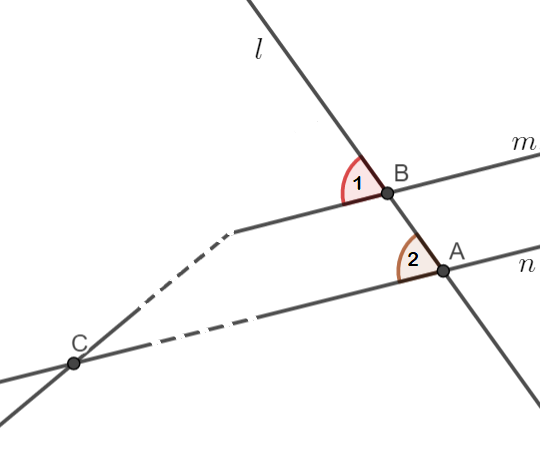
\includegraphics[width=0.27\textwidth]{反证法1.png}
\end{wrapfigure}
当原命题是“任何”、“不存在”这种全判断的时候,它的否定是“至少有一个”这种有判断。这时,使用反证法就可以对这个“有一个”
的特例进行论证,非常方便。

\begin{tm}\label{tm:2-0-0}
    两条直线$m,n$交另一条直线$l$于两点。如果同位角相等,那么$m,n$平行。
\end{tm}
\begin{proof2}
    使用反证法。命题“如果同位角相等,那么$m,n$平行”的否定是“有一对同位角相等,而且$m,n$不平行”。
    为了证明原命题是真的,我们假设它的否定是真的,然后推理得到矛盾。\\
    反设有一对同位角$\angle 1$和$\angle 2$相等,而且$m,n$不平行。设$m,n$的交点$C$在点$A$的一侧(如右图)。
    $\angle ACB + \angle 2$等于$\angle 1$的补角。但$\angle 1 = \angle 2$,
    所以$\angle ACB = 0^\circ$,这说明$m$和$n$重合而非平行。\\
    这就产生了矛盾!\\
    如果交点$C$在点$A$另一侧,通过类似推理可同样推出矛盾。\\
    这说明原命题的否定“有一对同位角相等,而且$m,n$不平行”是假的,因此原命题是真的。
\end{proof2}

反证法的好处在于,通过假设命题的否定为真,我们多了一个用来推理的条件。

\begin{xt}
    用反证法证明:\\
    \indent 1. 如果任一整数$n$的立方是奇数,那么$n$也是奇数。\\
    \indent 2. 所有奇数的平方除以$8$都余$1$。\\
    \indent 3. 证明垂距定理的逆命题:如果直线$l$外一点$P$到$l$上某点$Q$的距离不大于它到$l$上任何点的距离,
    那么$OQ \perp l$。
    动手做:\\
    \indent 补全定理\ref{tm:2-0-0}中根据“交点$C$在点$A$另一侧”推出矛盾的过程。
\end{xt}

\section{归纳法}
\begin{ex}\label{ex:2-2-0}
    观察并验证以下等式,你有什么发现?\\
    1. $1 + 3 = \frac12(3^2 - 1)$,$1 + 3 + 9 = \frac12(3^3 - 1)$,$1 + 3 + 9 + 27 = \frac12(3^4 - 1)$。\\
    2. $1 = \frac12(1+1)$,$1 + 2 = \frac22(1 + 2)$,$1 + 2 + 3 = \frac32(1 + 3)$。\\
    3. $\frac13 + \frac14 + \frac15 + \frac16 > \frac{9}{10}$,$\frac14 + \frac15 + \cdots + \frac{1}{9} > \frac{9}{10}$,
    $\frac15 + \frac16 + \cdots + \frac{1}{12} > \frac{9}{10}$。    
\end{ex}
从纷乱繁杂的事物中发现规律,是人类认识自然、改造自然的活动中不可缺少的一环。
归纳,就是试图用简单的规则概括已知的现象。比如,上面第一个例子中,我们可以归纳出这样的规律:
$$ \forall n \in \mathbb{N}, \,\,\, 1 + 3 + 3^2 + \cdots + 3^n = \frac{3^{n+1} - 1}{2}. $$
第二个例子中,我们可以归纳出:
$$ \forall n \in \mathbb{Z}^+, \,\,\, 1 + 2 + \cdots + n = \frac{n(n+1)}{2}. $$
第三个例子中,我们可以归纳出:
$$ \forall n \in \mathbb{Z}^+, \,\,\, \frac{1}{n+1} + \frac{1}{n+2} + \cdots + \frac{1}{3n} > \frac{9}{10}. $$
归纳得到的规律,并不总是正确的。比如,把$n=1$代入我们从第三个例子中归纳出来的不等式:
$$ \frac12 + \frac13 > \frac{9}{10}.$$
这个结论是错的。

怎样正确地归纳事物的规律呢?或者说,什么时候,我们可以确信归纳出的规律是正确的呢?
在漫长的数学研究中,人们认识到:
\begin{po}{\textbf{归纳公理}}
    设$P(n)$是一个含变量的命题,变量$n$可以是任意自然数。如果$P$满足以下两个条件:\\
    1. $P(0)$成立。\\
    2. 对每个自然数$n$,只要$P(n)$成立,$P(n+1)$就成立。\\
    那么,$P(n)$对任意自然数$n$都成立。
\end{po}
使用归纳公理的证明,也叫做用(数学)归纳法证明。用“数学”两个字,是为了和日常生活中凭有限经验归纳的做法区别开来。

以上三个例子中的规律,如何用归纳公理来论证呢?我们分别来写出过程。
\begin{proof2}{\textbf{第一个例子 }}
    命题$P(n)$:
    $$ 1 + 3 + 3^2 + \cdots + 3^n = \frac{3^{n+1} - 1}{2}. $$
    按照归纳公理,要论证命题对任意自然数$n$都成立,我们分别验证两个条件:\\
    1. $P(0)$可以写成:$1 = \frac{3 - 1}{2}$,显然成立。\\
    2. 假设$P(n)$对某个自然数$n$成立,我们来证明$P(n+1)$成立。\\
    $P(n+1)$可以写成:
    $$ 1 + 3 + 3^2 + \cdots + 3^{n+1} = \frac{3^{n+2} - 1}{2}. $$
    由于$P(n)$成立,$(1)$式左边的前$n+1$项可以写成$\frac{3^{n+1} - 1}{2}$,于是两边同时减去这一项,得到:
    \begin{align}
        3^{n+1} &= \frac{3^{n+2} - 1}{2} - \frac{3^{n+1} - 1}{2} \notag \\
        &= \frac{3\cdot 3^{n+1}}{2} - \frac{3^{n+1}}{2} \notag \\
        &= \frac{3\cdot 3^{n+1} - 3^{n+1}}{2} \notag \\
        &= \frac{2 \cdot 3^{n+1}}{2} = 3^{n+1} \notag
    \end{align}
    显然成立。因此,根据归纳公理,$P(n)$对任意自然数$n$都成立。    
\end{proof2}

我们可以看到,论证的时候,我们分别验证归纳公理要求的两个条件成立。从复杂的代数式到显然成立的等式,
我们用到了变量代换和因式分解的技巧。

\begin{proof2}{\textbf{第二个例子 }}
    命题$P$只对正整数有定义,所以我们要证明$P(n)$对所有正整数$n$成立。
    为此,我们稍微改变一下论证方式。\\
    命题$P(n)$:
    $$ 1 + 2 + \cdots + n = \frac{n(n+1)}{2}. $$
    按照归纳公理,要论证命题对任意自然数$n$都成立,我们分别验证两个条件:\\
    1. $P(1)$可以写成:$1 = \frac{1(1+1)}{2}$,显然成立。\\
    2. 假设$P(n)$对某个自然数$n$成立,我们来证明$P(n+1)$成立。\\
    $P(n+1)$可以写成:
    $$ 1 + 2 + \cdots + (n+1) = \frac{(n+1)(n+2)}{2}.  $$
    由于$P(n)$成立,$(1)$式左边的前$n$项可以写成$\frac{n(n+1)}{2}$,于是两边同时减去这一项,得到:
    \begin{align}
        n+1 &= \frac{(n+1)(n+2)}{2} - \frac{n(n+1)}{2} \notag \\
        &= \frac{n+1}{2}\left(n+2 - n\right) \notag \\
        &= \frac{n+1}{2} \cdot 2 = n+1 \notag
    \end{align}
    显然成立。因此,根据归纳公理,$P(n)$对任意正整数$n$都成立。    
\end{proof2}

\begin{proof2}{\textbf{第三个例子 }}
    命题$P(n)$:
    $$ \frac{1}{n+1} + \frac{1}{n+2} + \cdots + \frac{1}{3n} > \frac{9}{10}. $$
    我们已经验证过,$P(1)$不成立。现在利用归纳公理证明$P(n)$对大于等于$2$的自然数成立。
    为此,我们稍微改变一下论证方式。\\
    要论证命题对任意大于等于$2$的自然数$n$成立,我们分别验证两个条件:\\
    1. $P(2)$可以写成:
    $$\frac13 + \frac14 + \frac15 + \frac16 > \frac{9}{10}.$$
    计算可知等式左边等于$\frac{19}{20} > \frac{9}{10}$,因此$P(2)$成立。\\
    2. 假设$P(n)$对某个自然数$n$成立,我们来证明$P(n+1)$成立。\\
    $P(n+1)$可以写成:
    $$ \frac{1}{n+2} + \frac{1}{n+3} + \cdots + \frac{1}{3n+3} > \frac{9}{10}. $$
    由于$P(n)$成立,我们试着把上式左边用$P(n)$有关的式子表达出来,我们发现
    \begin{align}
        \frac{1}{n+2} + \frac{1}{n+3} + \cdots + \frac{1}{3n+3} =& \frac{1}{n+1} + \frac{1}{n+2} + \cdots + \frac{1}{3n} \notag \\
        &+ \frac{1}{3n+1} + \frac{1}{3n+2} + \frac{1}{3n+3} - \frac{1}{n+1} \notag 
    \end{align}
    而
    \begin{align}
        \frac{1}{3n+1} + \frac{1}{3n+2} + \frac{1}{3n+3} - \frac{1}{n+1} &>  \frac{1}{3n+3} + \frac{1}{3n+3} + \frac{1}{3n+3} - \frac{1}{n+1} \notag \\
        = \frac{3}{3n+3} - \frac{1}{n+1} = 0. \notag 
    \end{align}
    这说明:
    $$ \frac{1}{n+2} + \frac{1}{n+3} + \cdots + \frac{1}{3n+3} > \frac{1}{n+2} + \frac{1}{n+3} + \cdots + \frac{1}{3n}. $$
    $P(n)$告诉我们,上式右边大于$\frac{9}{10}$,所以上式左边也大于$\frac{9}{10}$。也就是说,$P(n+1)$成立。\\
    因此,根据归纳公理,$P(n)$对任意大于等于$2$的自然数$n$都成立。    
\end{proof2}
从第二、第三个例子可以看出,归纳公理可以换个“开头”使用。为什么可以这么做呢?让我们来理解归纳公理是如何告诉我们$P(n)$对
任意自然数$n$都成立的。

举例来说,我们知道$P(0)$成立,并且只要$P(n)$成立,$P(n+1)$就成立。现在我们想知道$P(100)$为何成立。
论证过程是这样的:只要$P(n)$成立,$P(n+1)$就成立,而$P(0)$成立,所以$P(1)$也成立。接下来,既然$P(1)$成立,
我们又可以得到$P(2)$成立。以此类推,经过$100$次这样的推理,我们就知道,根据$P(99)$成立,有$P(100)$成立。

使用归纳公理,就好比跑步。第一个条件告诉我们从哪里出发;第二个条件告诉我们,可以一步一步跑下去。
第二、第三个例子的证明里,我们换了一个“起跑线”,但论证了每步都能接到下一步。
于是,我们可以从$1$或$2$出发,“跑”到每个大于等于$2$的自然数$n$那里去。

\begin{sk}\label{sk:2-2-1}
    想一想:\\
    小强在证明的时候用了这样的归纳法:\\
    首先证明:$P(0)$成立。然后证明:对每个自然数$n$,只要$P(1), P(2), \cdots , P(n)$成立,那么$P(n+1)$也成立。
    根据以上两点,就可以说命题$P(n)$对任意正整数成立。\\
    你觉得这个推理方法对吗?
\end{sk}

\section{无穷}
做整数除法的时候,我们会遇到两种情况:除得尽和除不尽。列出竖式后,我们用被除数减去除数和商的积,得到余数。
如果某次得到的余数是$0$,就说除法除得尽。如果每次余数都不是$0$,我们就说除法除不尽。我们可以不断按照竖式除法的规则求余数,
但这个过程是无穷无尽的。

夜晚,仰望星空的时候,我们说星星是数不尽的,星星离我们无限遥远。郊游时,看着满地的鲜花,我们说花儿是数不完的。
是因为星星和花朵的数量太多,数起来太费时间,还是因为它们不可能数得完?是因为星星和我们的距离太远,没有测量的办法,
还是因为它们不可能被测量出来?多、远、大、久这些概念,是否有尽头?我们日常形容多、远、大、久等概念的时候,会用“无限”、
“无穷”、“无尽”这样的词来修饰,以表达夸张。到底“无限”、“无穷”、“无尽”是什么意思呢?

为了好理解,我们用数数作为例子:从$1$开始数数,每次加$1$:$1,\,\,2,\,\,3,\cdots$。
会不会到了某一步,我们无法再数下去呢?

如果从$1$数到$1'0000$,那么到了第$9999$步,我们就数完了。
如果从$1$数到$1000'0000$,那么到了第$999'9999$步,我们就数完了。

一般来说,如果要数的是前$n$个正整数,那么在第$n$步,我们就数完了,因为$n+1$乃至更大的数都不在前$n$个正整数里。

但是,如果要数的是全体正整数,那么我们可以一直数下去。因为每个正整数$n$后面的数:$n+1$都是正整数。
所以,全体正整数集合和前$1'0000$个正整数、前$1000'0000$个正整数或前$n$个正整数构成的集合不一样。

数学中,我们可以将集合分为两类。一类称为\textbf{有限}或\textbf{有穷},一类称为\textbf{无限}或\textbf{无穷}。
前$1'0000$个正整数、前$1000'0000$个正整数、前$n$个正整数这样的集合是有限或有穷的。
全体正整数、全体自然数这样的集合是无限或无穷的。

我们把前面“数数”的方法推广到一般的集合,判别集合有穷还是无穷。
一开始,集合所有的元素都是没数过的。
我们逐个来数它的元素:每次选择一个没数过的元素,
把它标记为数过的。这样,就说这个元素被数到了。
每个元素至多被数到一次,从没数过的元素变成数过的元素。

如果无论每次依什么规则选取元素,
数数过程都会因为没有没数过的数而停止,就说集合是有穷的,或集合元素的个数是有穷的。如果依照某个规则,数数过程不会停止,
就说集合是无穷的,或集合元素的个数是无穷的。

概括来说,数得尽的集合是有穷的,数不尽的集合是无穷的。我们把这种判别方法称为\textbf{数数原则}。

前面我们给正整数设计的数数规则就是一种不会停止的规则:选择上次数到的数加$1$得到的数。一方面,按照这个规则,
每次数到的数总是数过的数里最大的。另一方面,正整数加$1$总是正整数,所以按照规则,
用上次数到的数加$1$,就得到一个没数过的正整数。
按照数数原则,我们可以判定:全体正整数是无穷的。

依照同一个规则,我们也可以判定:全体自然数是无穷的。

对于前$n$个自然数的集合,我们可以证明它是有穷的。

记前$n$个自然数的集合为$X_n$,数数过程中,记第$i$步结束后所有没数过的数的个数为$G(i)$。
记一开始所有没数过的数的个数为$G(0)$,则$G(0) = n$。无论用什么规则,每一步结束后,没数过的数都少了一个,
即$G(i+1) = G(i) - 1$。于是,$G(n) = G(0) - n = 0$。第$n$步后,不再有没数过的数,数数过程只能停止。
根据数数原则,$X_n$是有穷的。

要注意的是,数数原则并不总要求每个数都被数过。如果集合是有穷的,按照定义,停止时所有的数都被数过了;
如果集合是无穷的,那么由于数数过程不会停止,不一定每个数都被数过。
比如,我们按照每次加$2$的方式给全体正整数的集合数数:
$1,3,5,\cdots$。这个过程不会停止,但偶数永远不会被数到。

\begin{sk}
    \mbox{}\\
    \indent 1. “除不尽”的例子中,什么是无穷的?\\
    \indent 2. 全体偶数是否是无穷的?全体整数是否是无穷的?全体有理数呢?你可以总结出什么规律?
\end{sk}

\chapter{方根和实数}

\section{方根}
减法是加法的逆运算,除法是乘法的逆运算,乘方有没有逆运算呢?

$3^2 = 9$,而$9$通过乘$2$次方的逆运算得到$3$。这个运算称为开$2$次方或开平方。

\textbf{开方}是乘方的逆运算。已知一个数的乘方和相应的指数,开方就得到原来的底数。
开方的结果称为\textbf{方根}。一个数开几次方,就得到几次方根。

开$1$次方得到的是自己。开$2$次方也叫开平方,结果叫平方根。开$3$次方也叫开立方,结果叫立方根。
一般来说,开$n$次方的结果叫$n$次方根。一般用$\sqrt[n]{\cdot}$表示开$n$次方运算。比如,
$5$开$3$次方记为$\sqrt[3]{5}$。为了方便,$n=2$时,一般忽略$\sqrt[2]{x}$中的$2$,直接记为$\sqrt{x}$。

开方是映射吗?我们知道$3^2 =9$,但同时也有$(-3)^2 =9$,那么可不可以说,$9$开平方得到$-3$呢?

为了让开方成为映射,我们约定:\textbf{方根总是正数}。这样,开方运算就定义了一个映射。

当$n$是偶数的时候,$n$次乘方运算的结果总大于等于零。因此,只有大于等于零的数可以开偶数次方,
负数无法开偶数次方。

当$n$是奇数的时候,$n$次乘方运算的结果可以大于或小于零,因此,正数和负数都可以开奇数次方。
$-1$的奇数次方仍是$-1$,因此$-1$开奇数次方也是$-1$。
这说明,互为相反数的,开奇数次方也互为相反数。

指数的加减意味着乘方的乘除,那么指数的乘除意味着什么呢?

考虑$2^{3\times 2} = 2^6$,$3\times 2 = 3 + 3$,于是$2^6 = 2^3 \times 2^3 = \left(2^3\right)^2$。

指数相乘表示乘方的乘方。比如,$2$的$3\times 2$次方等于$2$的$3$次方的$2$次方。
乘法满足交换律,故而$2$的$3$次方的$2$次方也等于$2$的$2$次方的$3$次方。

$4^{3\div 2}$意味着什么呢?

$3\div 2 \times 2 = 3$,所以我们希望$4^{3\div 2 \times 2} = 4^3$,也就是说,
$\left(4^{3\div 2}\right)^2 = 4^3$。
或者说,我们定义$4^{3\div 2}$为$4$的$3$次方再开$2$次方。
这样,我们可以定义一个数的分数次方。

显然,分数次方也不总是存在的,比如$4^{3\div 2}$之所以存在,是因为$4$的$3$次方大于等于零,可以开平方。
如果把$4$改为$-4$,$(-4)^{3\div 2}$是无法定义的。但如果把$2$换成某个奇数,比如$5$,那么$(-4)^{3\div 5}$是有定义的。

\begin{sk}\label{sk:3-0-0}
    $n$是奇数时,证明:\\
    1. 如果有理数$a > b$,那么$a^n > b^n$。\\
    2. 给定有理数$a, b$。如果$a^n > b^n$,那么$a > b$。\\
    3. 只要$a \neq b$,那么$\sqrt[n]{a} \neq \sqrt[n]{b}$(假设两者存在)。\\
    想一想:\\
    $(-3)^{2\div 2}$有意义吗?$n$为奇数和偶数时,$x \mapsto \sqrt[n]{x^n}$分别是怎样的函数?
\end{sk}

\section{无理数和实数}
学习反证法的时候,我们证明了这样一个结论:任何有理数的平方都不是$2$。
而上一节中,我们定义了开平方的运算。$2$开平方的结果记为$\sqrt{2}$,
于是我们有结论:$\sqrt{2}$不是有理数。

另一方面,$\sqrt{2}$是有意义的。勾股定理告诉我们,直角边长为$1$的等腰直角三角形,斜边长的平方等于$1^2+1^2=2$,
因此斜边长是$\sqrt{2}$。也就是说,等腰直角三角形斜边长度和直角边长度之比总是$\sqrt{2}$。

我们把能够表示为长度的数称为(正)实数。或者说,原点到数轴上任一点的距离,按正方向标记正负,
构成的集合,称为\textbf{实数}。

实数集合一般记为$\mathbb{R}$。

$\sqrt{2}$能够表示为长度或两点间的距离,所以$\sqrt{2}$是实数。但$\sqrt{2}$不是有理数。我们把这样的实数叫做\textbf{无理数}。

无理数有哪些呢?按照证明\ref{ex:2-0-1}的思路,只要自然数$n$不是完全平方数,$\sqrt{n}$总是无理数。另外,有理数之间的加减乘除总是有理数,所以:
\begin{tm}\label{tm:3-1-0}
    任一无理数和任何有理数进行有限次加减乘除(不包括乘以$0$),得到的结果仍然是无理数。
\end{tm}
\begin{proof2}
    用反证法证明。反设原命题的否定为真:存在某个无理数$t$和某些有理数经过有限次加减乘除(不包括乘以$0$)
    后得到的是有理数$r$。那么,
    $r$经过这些与有理数的加减乘除的逆运算(不包括除以$0$),得到无理数$t$。但我们知道,有理数之间的加减乘除运算
    总得到有理数。这就造成了矛盾!\\
    因此,原命题为真:任何无理数和任何有理数进行有限次加减乘除(不包括乘以$0$),得到的结果仍然是无理数。
\end{proof2}
比如,$\sqrt{2}+1$,$\frac{\sqrt{7} - 2}{5}$等等都是无理数。

\begin{xt}\label{xt:3-1-0}
    证明:\\
    1. 当$n,m$是正整数时,$\sqrt[n]{m}$要么是整数,要么是无理数。\\
    2. $\frac{2 - \sqrt{3}}{\sqrt{3} - 1}$是无理数。\\
    下面的式子能否表达成更简单的方式?\\
    1. $\sqrt{8 - 2\sqrt{7}}$\\
    2. $\sqrt[3]{26 - 15\sqrt{3}}$
\end{xt}

\section{二次方根}
有理数开平方的结果,叫做\textbf{二次方根}。前面提到的$\sqrt{2}$就是二次方根。
只要有理数$q$大于等于$0$,就存在二次方根$\sqrt{q}$。按照二次方根的定义,
$$\forall q\in\mathbb{Q}^+, \quad \left(\sqrt{q}\right)^2 = q.$$

二次方根有多大?拿出尺子量一量,$\sqrt{2}$厘米大概有多长?(如何画出$\sqrt{2}$厘米?)

要求$\sqrt{2}$的大小,我们可以采用逐步逼近的办法。首先,$\sqrt{2}$是直角边为$1$的等腰直角三角形的斜边长,
因此,$\sqrt{2}$大于直角边长:$1$,小于另外两边之和:$2$。
接下来,我们可以用\textbf{二分法},尝试找到一个近似的值。

第一步:使用$1$和$2$的平均数:$1.5$。比较$1.5$和$\sqrt{2}$的大小:
$$ 1.5 - \sqrt{2} = \frac{1.5^2 - \left(\sqrt{2}\right)^2}{1.5 + \sqrt{2}} $$
而$1.5^2 = 2.25 > 2 = \left(\sqrt{2}\right)^2$,所以
$$ \frac{1.5^2 - \left(\sqrt{2}\right)^2}{1.5 + \sqrt{2}} > 0,$$
即$1.5 > \sqrt{2}$。

第二步:使用$1$和$1.5$的平均数:$1.25$。比较$1.25$和$\sqrt{2}$的大小.使用如上办法,得到
$1.25 < \sqrt{2}$。

依此法重复,每步得到$\sqrt{2}$的上下限:$a < \sqrt{2} < b$,然后比较上下限的平均数$\frac{a+b}{2}$和
$\sqrt{2}$的大小。如果$\frac{a+b}{2}$比$\sqrt{2}$大,就用$\frac{a+b}{2}$代替$b$,得到一个新上限;
如果$\frac{a+b}{2}$比$\sqrt{2}$小,就用$\frac{a+b}{2}$代替$a$,得到一个新下限。然后对新得到的上下限进行下一步。
每步结束后,上下限之间的差距都缩小到之前的一半。于是,$n$步之后,上下限之间的差距就会缩小到$\frac{1}{2^n}$。
比如,$10$步之后,上下限之间的差距是$\frac{1}{1024}$,具体是:$1.4140625 < \sqrt{2} < 1.4150390625$。

一般来说,二次方根$\sqrt{q}$也可以用类似的方法求得。
\begin{sk}\label{sk:3-2-0}
    以上方法中,为什么需要取平均数?有没有别的方法更新上下限?
\end{sk}

二次方根的乘除运算:给定两个有理数$q$和$r$,它们的二次方根的乘积满足:
\begin{align}
    \left(\sqrt{q}\sqrt{r}\right)^2 &=  \left(\sqrt{q}\sqrt{r}\right)\left(\sqrt{q}\sqrt{r}\right) \notag \\
    &= \left(\sqrt{q}\sqrt{q}\right)\left(\sqrt{r}\sqrt{r}\right) = qr \notag 
\end{align}
所以
$$\sqrt{q}\sqrt{r} = \sqrt{qr}.$$
同样,$r \neq 0$时,
$$\frac{\sqrt{q}}{\sqrt{r}} = \sqrt{\frac{q}{r}}.$$

\begin{xt}\label{xt:3-2-0}
    \mbox{}\\
    以下的二次方根大约有多大(精确到两位小数)?\\
    \indent 1. $\sqrt{3}, \sqrt{5}, \sqrt{7}$.\\
    \indent 2. $\sqrt{1.6}, \sqrt{9.2}$.\\
    \indent 3. $\sqrt{\frac{5}{4}}, \sqrt{\frac{7}{3}}$.\\
    算一算:\\
    \indent 1. $\sqrt{2.4} \cdot \sqrt{9.6}$\\
    \indent 2. $\sqrt{\frac{1.78}{0.92}}.$
\end{xt}

\chapter{图形和坐标}
\section{平面直角坐标系}
我们已经了解了数轴的概念。数轴把数和形状结合了起来,
给定了一条直线,确定了原点、单位长度和正方向,我们就可以把数
和直线上的点联系起来。

\begin{sk}\label{sk:4-0-0}
    如何在数轴上找到$\frac{7}{11}$对应的点?$\sqrt{2} - 1$呢?
\end{sk}

数轴可以把直线上的点和数联系起来,通过数的大小,确定点的位置关系。
规定了正方向之后,我们可以说,如果数轴上三点$A,B,C$对应的数$a,b,c$满足$a < b < c$,
那么点$B$就在$A$和$C$之间,或者说在线段$AC$上。如果$a < c < b$,那么$B$就不在线段$AC$上。

在平面里,能否把点和数联系起来,方便地确定点的位置呢?

从数轴的原点$O$出发,我们作另一条直线。在这条直线上,我们沿用$O$为原点,
沿用单位长度,并选择一个正方向。这样,我们就建立了一个\textbf{坐标系}。
换句话说,把两条数轴放在一起,让原点重合,就得到一个坐标系。
我们一般让新数轴与原数轴垂直,这样得到的坐标系叫做\textbf{直角坐标系}。
我们把原来的数轴叫做$x$\textbf{轴},
把新数轴叫做$y$\textbf{轴}。直角坐标系可以简记为$Oxy$或$xOy$。
两个坐标轴把平面分成四部分。我们把右上的部分称为第一象限,然后沿逆时针顺序,
把左上、左下、右下部分分别称为第二、三、四象限。

\begin{wrapfigure}[13]{r}{0.62\textwidth} %this figure will be at the right
    \vspace{-30pt}
    \centering
    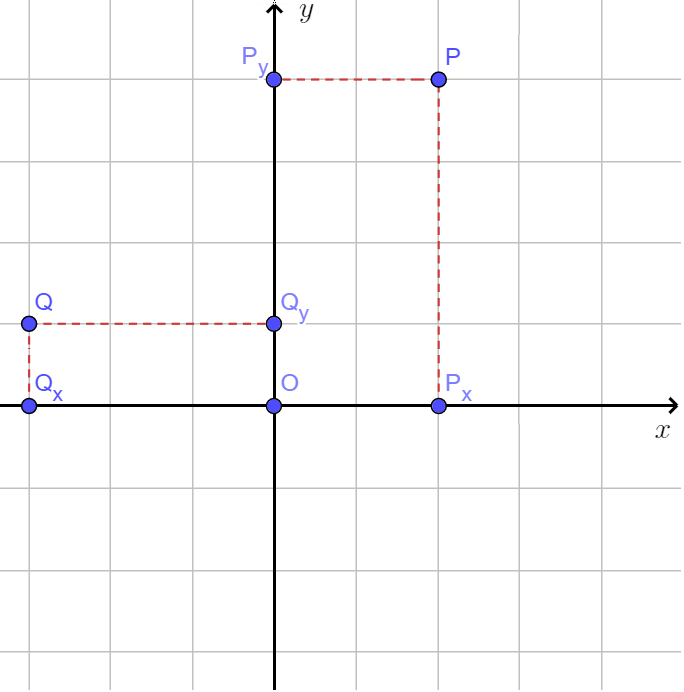
\includegraphics[width=0.6\textwidth]{坐标系2.png}
    \caption*{\texttt{平面直角坐标系}}
\end{wrapfigure}

直角坐标系如何表示平面中一点的位置呢?

设$P$是平面中一点。过$P$分别作$y$轴和$x$轴的平行线,交$x$轴和$y$轴于点$P_x$和$P_y$。
$P_x$和$P_y$分别对应数轴上的数$x_P$和数$y_P$。我们就用这两个数组成的数对$(x_P, y_P)$表示点$P$。

注意:数对和集合不同。首先,它是由两个数构成的,这两个数可以相同。其次,数对规定了这两个数的顺序,
顺序改变了,数对也改变了。比如$(1,2)$和$(2,1)$是两个不同的数对。

用这种方法表示平面中的点,有什么好处呢?

首先,我们可以发现,一个点确定一个数对,反过来,一个数对也恰好确定平面中一个点。给定一个数对$(x_P, y_P)$,
数$x_P$在$x$轴上确定唯一一点$P_x$,$y_P$在$y$轴上确定唯一一点$P_y$,于是,过$P_x$作$y$轴平行线,
过$P_y$作$x$轴平行线,交于唯一一点$P$。不会有两点对应同一个数对,也不会有两个数对对应同一个点。

我们把点到数对的映射记为$f$,把数对到点的映射记为$g$,$f$和$g$这样的映射称为\textbf{一一映射},
也叫做\textbf{双射}。

其次,给定一点$P$,我们可以方便地知道它到原点的距离。考虑$\triangle OP_xP$,它是直角三角形,
$\angle OP_xP$是直角。因此,根据勾股定理,
$$|OP|^2 = |OP_x|^2 + |P_xP|^2.$$
$|OP_x| = |a|$,而$\triangle OP_xP\cong \triangle PP_yO$,
所以$|P_xP| = |OP_y| = |b|$,也就是说,
$$ |OP|^2 = a^2 + b^2.$$

任意两点$P$和$Q$之间的距离也可以用类似的方法计算。把上面论证中的$O$改为$Q$,使用全等三角形的性质,可以得到
$$|PQ|^2 = |P_xQ_x|^2 + |P_yQ_y|^2.$$
根据数轴上的运算法则,设$P$和$Q$分别对应数对$(x_P, y_P)$和$(x_Q, y_Q)$,
那么$|P_xQ_x| = |x_P- x_Q|$,$|P_yQ_y| = |y_P- y_Q|$。因此
$$ |PQ|^2 = (x_P- x_Q)^2 + (y_P - y_Q)^2,$$
也就是说,平面中$P$和$Q$两点的距离(线段$|PQ|$的长度)是:
$$ |PQ| = \sqrt{(x_P- x_Q)^2 + (y_P - y_Q)^2}.$$
我们把数对$(x_P, y_P)$叫做点$P$在坐标系$Oxy$上的\textbf{坐标},把$x_P$叫做它的\textbf{横坐标},
$y_P$叫做它的\textbf{纵坐标}。
\begin{xt}\label{ex:4-0-0}
    证明$|PQ|^2 = |P_xQ_x|^2 + |P_yQ_y|^2.$
\end{xt}

\section{轴对称和中心对称}
\begin{wrapfigure}[6]{r}{0.3\textwidth} %this figure will be at the right
    \vspace{-30pt}
    \centering
    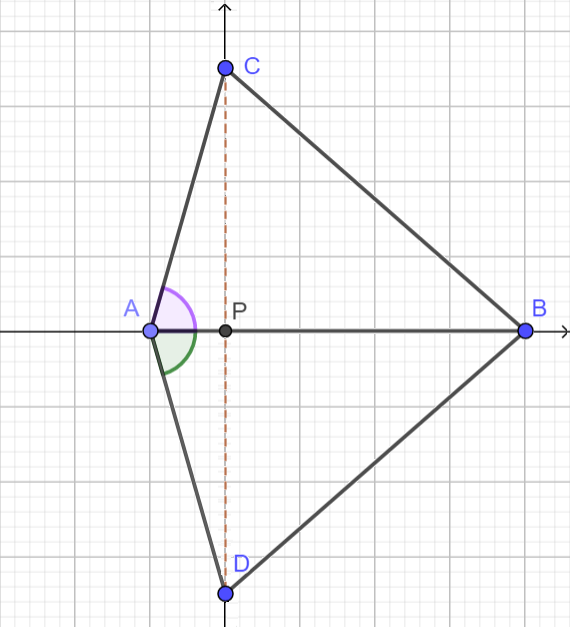
\includegraphics[width=0.288\textwidth]{坐标系3.png}
\end{wrapfigure}

“对称”是生活中常用的词。数学中,对称也是很重要的概念。讨论全等三角形的时候,我们用右图中的方法
证明“边角边”定理。图中的$ABC$和$ABD$就是对称的。可以注意到,直线$AB$有特殊的地位。
如果把$\triangle ABC$沿着$AB$从上往下“翻过来”,恰好就是$\triangle ABD$。这样的对称关系称为轴对称。
我们说$\triangle ABC$和$\triangle ABD$是关于直线$AB$对称,直线$AB$称为\textbf{对称轴}。

对称和角有密切关系。比如,$\triangle ABC$和$\triangle ABD$是关于直线$AB$对称,
而$\angle CAB$和$\angle DAB$是一对相反的角。角关于自己的一条边所在直线作对称,得到的是相反的角。

借助平面直角坐标系,我们可以更好地理解轴对称。比如,我们把直线$AB$设为$x$轴,把$P$点设为原点,
以射线$AB$的方向为正方向;把直线$CD$设为$y$轴,以射线$PC$的方向为正方向。这样建立的直角坐标系中,
设$C$的坐标是$(0, x_C)$,那么$D$的坐标就是$(0, -x_C)$。同样,设$\triangle ABC$某条边上任意一点
的坐标是$(a, b)$,那么$\triangle ABD$对应的边上也会有一点,坐标是$(x, -y)$,反之亦然。

一般来说,平面中一点$P = (a, b)$关于$x$轴的轴对称是点$P' = (x, -y)$。它们的横坐标相同,纵坐标互为相反数。
过$P$作$x$轴的垂线,垂足为$M = (a,0)$。延长$PM$到$P'$,使得$|PM| = |MP'|$,就得到$P'$。

给定平面中一点$P$和一条直线$l$,$P$关于$l$的对称点也可以依法作出。以$l$为$x$轴,$P$的横坐标和它的对称点
相同,纵坐标和它的对称点相反。

简单来说,说两点关于直线对称,就是说直线是两点连成线段的垂直平分线。

\begin{wrapfigure}{r}{0.5\textwidth} %this figure will be at the right
    \vspace{-15pt}
    \centering
    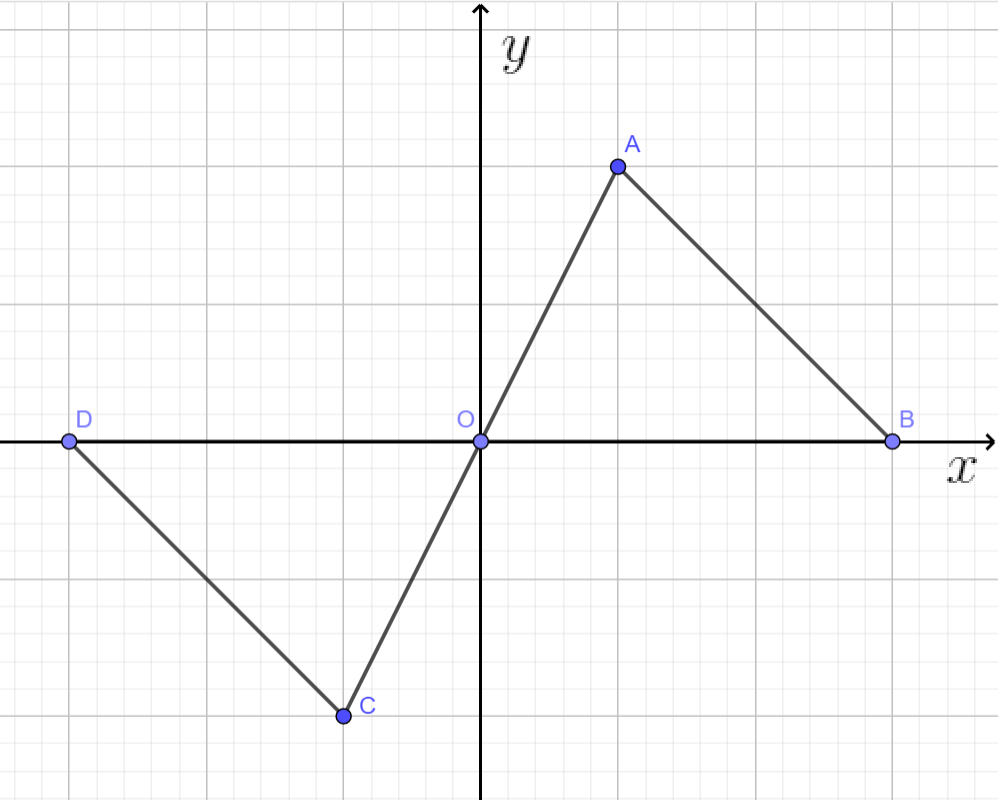
\includegraphics[width=0.5\textwidth]{轴对称1.png}
\end{wrapfigure}

除了关于直线的对称,图形还可以关于点对称。证明三角形外角等于另外两内角之和的时候,
我们构造了类似右图的形状。图中的$\triangle ABO$和$\triangle CDO$是全等三角形。
按照图中构建的直角坐标系,点$A$的坐标是$(1,2)$,点$C$的坐标是$(-1, -2)$;
点$B$的坐标是$(3,0)$,点$D$的坐标是$(-3, 0)$。设$\triangle ABO$某边上一点坐标是$(a, b)$,
那么在$\triangle CDO$对应边上可以找到一点,坐标是$(-a, -b)$,反之亦然。
也就是说,把一个三角形的横坐标和纵坐标都取相反数,就得到另一个三角形。

图中最特殊的一点当属点$O$。它的坐标是$(0,0)$,横坐标和纵坐标都取相反数,还是它自己。
我们说$O$是对称的中心。我们把这样的对称关系称为\textbf{中心对称},$\triangle CDO$与$\triangle ABO$关于$O$对称。
$\triangle CDO$是$\triangle ABO$关于$O$的对称图形,反之亦然。

给定平面中一点$P$和中心点$O$,延长$PO$到点$P'$,使得$|PO| = |OP'|$,那么$P'$就是$P$关于$O$的对称点。

简单来说,说两点关于一点$O$对称,就是说$O$是两点连成线段的中点。

对于角来说,如果中心点是角的顶点,那么角的对称是它的对顶角,因此大小和它相等。

\begin{sk}\label{sk:4-1-0}
    \mbox{} \\
    \indent 1. 三角形关于直线的对称图形与它自己有什么关系?\\
    \indent 2. 证明:角的轴对称图形是大小相反的角。\\
    \indent 3. 直角坐标系中,两点关于点$(4,3)$对称。这两点的坐标有什么关系?\\
    \indent 4. 三角形关于一点的对称图形,与它自己有什么关系?\\
    \indent 5. 证明:角的中心对称图形是大小相等的角。
\end{sk}

\section{对称之间的关系}
给定直角坐标系$xOy$,考虑关于$x$轴的轴对称。它把平面中每个点都对应到平面中另一点(可能重合)。
把平面所有点视作集合,记作$\mathcal{P}$,那么关于$x$轴的轴对称就是一个从$\mathcal{P}$到$\mathcal{P}$的映射。
我们把从一个集合到自身的映射叫做\textbf{变换}。为了方便,关于$x$轴的轴对称变换记作$\alpha$:
$$ \alpha (a, b) = (a, -b).$$
同理,关于$y$轴的轴对称也是从$\mathcal{P}$到$\mathcal{P}$的变换,我们把它记作$\beta$:
$$ \beta (a, b) = (-a, b).$$
点$(a, b)$经过$\alpha$,变为$(a, -b)$,再经过$\alpha$,又变回自身。
同样,$(a, b)$经过$\beta$,变为$(-a, b)$,再经过$\beta$,也再次变回自身。

如果$(a, b)$经过$\alpha$变换,再经过$\beta$,就变成$(-a, -b)$,也就是关于原点的中心对称点。
如果先经过$\beta$变换,再经过$\alpha$,$(a, b)$也变成$(-a, -b)$。
也就是说,关于两个坐标轴的轴对称变换叠加,等于做了关于原点的中心对称变换:$\gamma$。

把每个点对应到自身的变换,称为恒等变换,记为$\iota$。考虑$\iota$、$\alpha$、$\beta$和$\gamma$。
它们相互叠加,得到的结果是什么?你能补全下面的表格吗?
\begin{center}
    \begin{tabular}{  | p{2em}<{\centering} | p{2em}<{\centering} | p{2em}<{\centering} | p{2em}<{\centering} | p{2em}<{\centering} | }
        \hline
        $\circ$ & $\iota$ & $\alpha$ & $\beta$ & $\gamma$ \\ [0.5ex] 
        \hline
        $\iota$ &  &  &  &  \\  
        \hline
        $\alpha$ &  & $\iota$ & $\gamma$ &  \\  
        \hline
        $\beta$ &  & $\gamma$ & $\iota$ &  \\  
        \hline
        $\gamma$ &  &  &  &  \\ 
        \hline 
    \end{tabular}
\end{center}
$\iota$、$\alpha$、$\beta$和$\gamma$相互叠加,有什么规律?如果用$\circ$表示变换的叠加,
比如$\alpha \circ \beta$表示先经过$\beta$变换,再经过$\alpha$变换。那么$\circ$之于对称变换和
乘法之于数有什么共同之处?又有什么不同之处?据你所知,有什么概念和$\iota$、$\alpha$、$\beta$和$\gamma$的关系相似吗?

\begin{sk}\label{xt:4-2-0}
    \mbox{}\\
    1. 等边三角形有几个对称轴?等腰三角形呢?是否有三角形恰好有两个对称轴?\\
    2. 直角坐标系$xOy$中,设$OA$是$\angle xOy$的平分线,直线$OB$垂直于$OA$,
    用$v$和$w$分别表示以$OA$和$OB$的对称轴的轴对称变换。它们之间有什么关系?它们和$\iota$、$\alpha$、$\beta$和$\gamma$
    又有什么关系?
\end{sk}

\chapter{函数初步(上)}
函数是把数量对应到数量的映射。函数的出发集和到达集都是$\mathbb{N}$、$\mathbb{Q}$这样的数集。

作为映射,函数用来描述数与数之间的关系。如何理解一个函数呢?对于定义域是有限集合的函数,
我们可以用穷举法,列出定义域中所有元素在到达集里对应的值。对于定义域是无穷集合的函数,我们就没法
使用穷举法了。

理解函数,是数学中非常重要而困难的活动。为了理解$\mathbb{N}$、$\mathbb{Q}$、$\mathbb{R}$等无穷
集合上的函数,数学家们发明了各种各样的手段。从十九世纪开始,这些手段逐渐演变成一门学科,叫做
分析学。

数学家们最早分析的,是定义在整数和实数集合上的函数。前者被称为数列或级数,后者被称为实变函数。
这两种函数和日常生活联系最紧密。下面我们先来学习实变函数。

最简单的分析方法,是从一类或几类最简单的函数入手,然后研究别的函数和这些函数有什么共同点,
能否把我们在简单函数上理解到的东西应用在更多函数上。我们把入手研究的函数称为初等函数或基本函数。
如果初等函数选得好,我们能通过它们的性质,理解更多的函数。

\section{正比例函数}
我们知道,每个代数式都确定了一个函数,相应的代数式叫做函数的\textbf{表达式}或\textbf{解析式}。
可以用简单代数式表达的函数,叫做\textbf{初等函数}。
其中,常数对应的是\textbf{常函数}。常函数是把定义域中的元素对应到同一个常数的函数。
比如:$x\mapsto 1$就是一个常函数,它把所有元素对应到常数$1$。常函数一般用相应的常数标记,
比如,$x\mapsto 1$可以记作$1$。

另一种函数是\textbf{恒等函数}。它是代数式$x$对应的函数,把定义域中的元素对应到自身。
恒等函数一般记作$\mathrm{I}$或$\iota$,即$\mathrm{I}:x \mapsto x$。

从恒等函数出发,我们来了解正比例函数。

\textbf{正比例函数},是从正面描述比例关系的函数。介绍图形的相似关系的时候,我们提到了比例关系。
比例关系也叫倍数关系,是一种常见的数量关系。比如,两个三角形$\triangle ABC$和$\triangle A'B'C'$相似,那么
对应的边长成比例:
$$ \frac{|AB|}{|A'B'|} = \frac{|AC|}{|A'C'|} = \frac{|BC|}{|B'C'|} = k.$$
我们把$k$称为\textbf{比例系数}。比例系数确定时,边长的关系就是正比例关系,对应的映射叫正比例函数。
一般来说,正比例函数是这样的:
$$ x \mapsto kx$$
也就是把自变量$x$对应为它的$k$倍。比如,$x \mapsto 3x$就是一个正比例函数。
恒等函数其实就是比例系数为$1$的正比例函数。

设有正比例函数$f: x\mapsto kx$。当$k>0$的时候,$x$的值越大,$f(x)$也越大。
$k<0$的时候,$x$的值越大,$f(x)$越小。$k=0$的时候,无论$x$取值,$f(x)$的值总等于$0$。
$k$的正负对函数的性质有本质影响。

\begin{sk}\label{sk:5-0-0}
    生活中有哪些成比例的数量关系?如何用正比例函数表示这些关系?
\end{sk}

\begin{wrapfigure}{r}{0.35\textwidth} %this figure will be at the right
    \vspace{-10pt}
    \flushright
    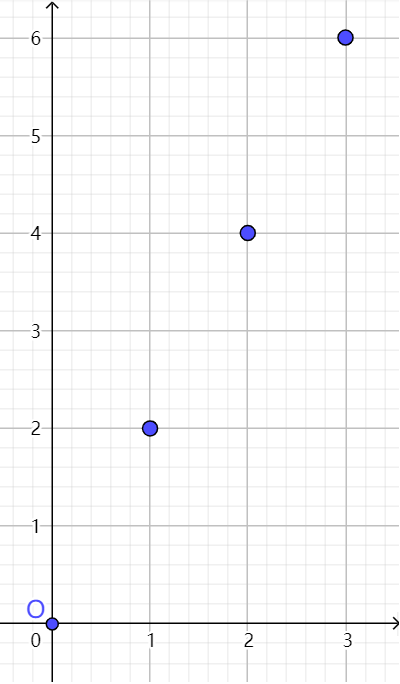
\includegraphics[width=0.32\textwidth]{正比例0.png}
\end{wrapfigure}

有没有更直观的方式可以了解正比例函数呢?我们可以用图形来表示正比例函数。

用函数$f: x \mapsto 2x$做例子。在平面中建立直角坐标系$xOy$。
自变量$x$取值为$1$的时候,$f(x)$的值为$2\cdot 1 = 2$。我们用点$(1, 2)$表示这个对应关系。
横坐标用来表示自变量$x$,纵坐标用来表示函数值$f(x)$。
同样地,$x$取值为$0,2,3$的时候,$f(x)$的值为$2\cdot 0 = 0$,$2\cdot 2 = 4$,$2\cdot 3 = 6$。
我们分别用点$(0,0)$、$(2,4)$和$(3,6)$表示这些关系。

如果我们让自变量取更多的值,就得到更多的点:$(x, f(x))$。所有点$(x, f(x))$构成的图形,
称为函数$f$的\textbf{图像}。

回到函数$f: x \mapsto 2x$,观察$(0, 0)$、$(1, 2)$、$(2,4)$和$(3,6)$点,我们发现,它们都在一条直线上。
可以猜测,$(x, f(x))$总在这条直线上,这条直线上的点也必然可以写成$(x, f(x))$的形式。也就是说,
函数$f$的图像是一条直线。

\begin{wrapfigure}[8]{r}{0.4\textwidth} %this figure will be at the right
    \vspace{-10pt}
    \flushright
    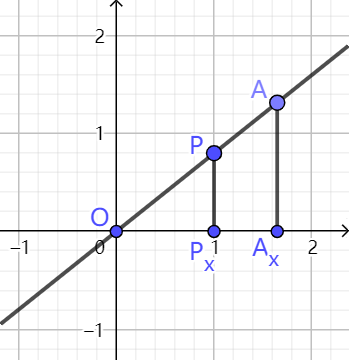
\includegraphics[width=0.35\textwidth]{正比例1.png}
\end{wrapfigure}

下面我们来证明这一点。

\begin{tm}\label{tm:5-0-0}
    正比例函数的图像是一条过原点的直线。
\end{tm}
\begin{proof2}
    设有正比例函数$f: x \mapsto kx$,其中$k$是比例系数。我们证明:$f$的图像是一条经过原点的直线。\\
    首先,$f(0) = k\cdot 0 = 0$。所以原点$O$可以写成$(0, f(0))$,因此在函数的图像上。\\
    其次,$f(1) = k\cdot 1 = k$,因此点$P = (1, k)$在图像上。\\
    设$O,P$确定的直线为$l$,下面证明,$f$的图像就是$l$。\\
    首先考虑$k > 0$的情况。这时候,$P$在第一象限。
    对任意数$a$,考虑点$A = (a, f(a)) = (a, ka)$。当$a$是正数的时候,$A$也在第一象限。
    当$a < 0$的时候,$A$在第三象限。\\
    按照定义,分别过点$A$和$P$作$y$轴的平行线,
    交$x$轴于$A_x = (a, 0)$和$P_x = (1, 0)$两点,那么$|P_xP| = k$,$|A_xA| = ka$,$|P_xO| = 1$,
    $|A_xO| = a$。而$\angle PP_xO = \angle AA_xO = 90^\circ$。所以,根据“边角边”,
    $\triangle PP_xO \simeq \triangle AA_xO$。这说明$\angle A_xOA = \angle P_xOP$。
    $a>0$时,$O,P,A$都在$\angle A_xOA$的终边上。$a<0$时,$A$和$P$分别在$O$两侧,射线$OA$和$OP$组成直线$l$。
    两种情况下,$A$都在直线$l$上。\\
    另一方面,如果$A = (x_A, y_A)$是$l$上一点,那么类似作出$A_x$和$P_x$,可以证明$\triangle PP_xO \simeq \triangle AA_xO$。
    于是
    $$ \frac{|A_xA|}{|A_xO|} = \frac{|P_xP|}{|P_xO|} = k.$$
    也就是说$|y_A| = k|x_A|$。由于直线$l$只经过第一、三象限,$x_A, y_A$要么同时是正数,要么同时是负数。
    因此总有$y_A = kx_A$。这就说明,$A$也在函数$f$的图像上。\\
    综上所述,$k>0$时,函数$f$的图像就是直线$l$。\\
    再考虑$k<0$的情况,这时$P$在第二象限,直线$l$经过第二、四象限。可以观察到,
    $l$关于$x$轴的对称图像就是$k>0$的情况。于是,通过类似推理,可以证明函数$f$的图像就是直线$l$。\\
    最后考虑$k=0$的情况,这时$f$就是常函数$x\mapsto 0$。于是对任意数$x$来说,$(x, f(x)) = (x, 0)$。
    于是它的图像就是$x$轴:一条过原点的直线。
\end{proof2}

直角坐标系把函数和图形联系了起来,让我们有了一种直观理解函数的方法。一般来说,
我们无法根据函数的定义轻易画出函数的图像。如果已知函数的图像,我们可以对函数有深入的了解。
比如,给定自变量的取值,我们可以直观地确定函数的值。

正比例函数的图像是一条过原点的直线。观察函数的图像,我们可以总结正比例函数的一些基本性质。

设有正比例函数$f: x\mapsto kx$。
对同样的元素$x$,$x>0$时,$k$越大,$f(x) = kx$也越大;$x<0$时,$k$越大,$f(x)$越小。
观察函数图像,可以发现,如果$k>0$,那么$k$越大时,$f$对应的曲线越“贴近”$y$轴,或者说越“陡峭”,
反之,$k$越接近$0$,$f$对应的曲线就越“贴近”$x$轴,或者说越“平坦”。而如果$k<0$,那么$k$越小时,
$f$对应的曲线越“贴近”$y$轴,或者说越“陡峭”,
反之,$k$越接近$0$,$f$对应的曲线就越“贴近”$x$轴,或者说越“平坦”。

讨论函数$f$的图像时,我们把$k$称为相应直线的\textbf{斜率},它决定了正比例函数对应的直线有多斜。

\begin{xt}\label{xt:5-0-0}
    完成定理\ref{tm:5-0-0} 中$k<0$的部分。
\end{xt}

\section{一次函数}
从正比例函数出发,我们还可以得到一次函数。
可以注意到,恒等函数和正比例函数分别对应一元一次式$x$和$kx$。一般来说,一元一次式
可以写成$ax+b$的形式。我们把形如$x \mapsto ax + b$的函数称为一次函数。其中的$a$仍然称为斜率,
$b$称为相应直线的\textbf{截距}。$b=0$的时候,一次函数就是正比例函数。$a=0$的时候,一次函数就是常函数。

如何从常函数和正比例函数得到一次函数呢?我们可以定义函数的四则运算。

设有函数$f$和$g$,两者定义域一致,
那么可以定义一个新函数$h$:对定义域中的任意元素$x$,$h(x) = f(x) + g(x)$。这样的函数$h$称为$f$和$g$的和函数,
简称$f$和$g$的和,记为$f + g$。类似可以定义$f$和$g$的差函数和积函数,分别记为$f - g$和$f\cdot g$。如果函数$g$
总不为$0$,那么还可以定义$f$和$g$的商函数:$h(x) = f(x) \div g(x)$,记为$f \div g$或$\frac{f}{g}$。

设有常函数$x\mapsto b$和正比例函数$x\mapsto ax$,那么它们的和就是一次函数$x\mapsto ax + b$。
如果从常函数$x\mapsto 1$和恒等函数$\mathrm{I}$出发,那么前者需要乘以$b$,后者需要乘以$a$。
于是,一次函数$x \mapsto ax + b$可以记为$a\mathrm{I} +b$。

\begin{wrapfigure}[12]{r}{0.35\textwidth} %this figure will be at the right
    \vspace{-10pt}
    \flushright
    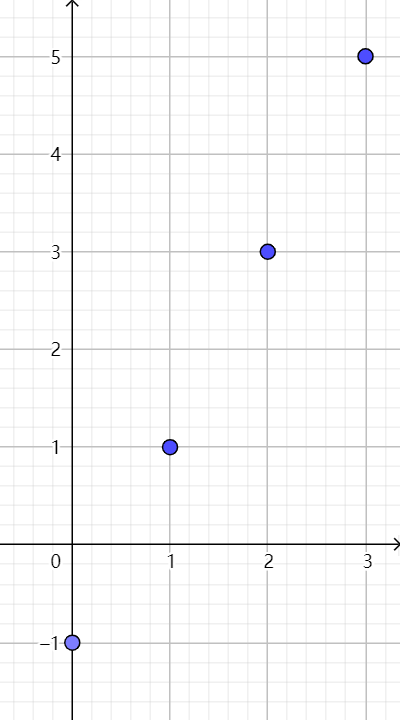
\includegraphics[width=0.32\textwidth]{一次函数1.png}
\end{wrapfigure}

可以发现,我们没有区分函数乘以函数和函数乘以常量。这是因为在函数的四则运算中,常函数可以看作和常数一样。
比如,给函数加上$x\mapsto 1$和加上$1$,意义是一样的。

一次函数的图像是怎样的呢?我们可以通过具体的例子来观察。设有一次函数$f: x\mapsto 2x - 1$。
通过描点可知,点$(0, -1)$、$(1, 1)$、$(2, 3)$、$(3, 5)$在函数的图像上。
用证明正比例函数的方法,我们可以证明:

\begin{tm}\label{tm:5-1-0}
    一次函数的图像是一条直线。
\end{tm}

一般来说,一次函数$x\mapsto ax + b$的图像是一条经过$(0, b)$的直线。$(0, b)$是直线和$y$轴的交点,
在数轴上对应$b$。$b>0$时,直线和$y$轴交于$x$轴上方,$a>0$时,经过第一、二、三象限,$a<0$时,经过第一、二、四象限。
$b<0$时,直线和$y$轴交于$x$轴下方,$a>0$时,经过第一、三、四象限,$a<0$时,经过第二、三、四象限。

\begin{xt}
    证明定理\ref{tm:5-1-0}:一次函数的图像是一条直线。
\end{xt}

\section{直线与平移}
上一节的例子中,一次函数$f: x\mapsto 2x - 1$和正比例函数$g: x\mapsto 2x$相差一个常函数$1$。
我们来看它们的图像的差别。

$f$和$g$定义域一致。对任意$x$,$f(x)$总比$g(x)$少$1$。或者说,$f$的图像在$g$的图像“下方”。
如果把$g$的图像中的每一点$(x, y)$都移到点$(x, y-1)$,就得到$f$的图像。

除此之外,还可以从另一个角度来看:对任意$y$,使得$f(x)=y$的$x$值总比使得$g(x)=y$的$x$值多$0.5$。
比如,对$y=3$来说,$f(2)=3$,$g(1.5)=3$。$2=1.5+0.5$。或者说,$f$的图像在$g$的图像“右边”。
如果把$g$的图像中的每一点$(x, y)$都移到点$(x+0.5, y)$,也能得到$f$的图像。

我们把这一类变换称为\textbf{平移}。沿$x$轴平移$x_0$个单位,就是:
$$ (x, y) \mapsto (x+x_0, y),$$
沿$y$轴平移$y_0$个单位,就是:
$$ (x, y) \mapsto (x, y+y_0).$$
这两个变换也可以合并。沿$x$轴平移$x_0$个单位,再沿$y$轴平移$y_0$个单位,就是:
$$ (x, y) \mapsto (x+x_0, y+y_0).$$
要注意的是,这两个变换的顺序是可以交换的,谁先谁后并不影响结果。

两次平移变换合并而成的变换,也叫做平移。每个平移,可以对应平面上一个点。沿$x$轴平移$x_0$个单位,
对应$(x_0, 0)$。沿$y$轴平移$y_0$个单位,对应$(0, y_0)$。合并的平移,对应$(x_0, y_0)$。
反过来,平面中任何点$(x_0, y_0)$,都可以对应一个平移:它的效果是把原点移到$(x_0, y_0)$。
所以,当我们说平移的时候,总说关于某个点的平移。

对一般的一次函数$x\mapsto ax+b$来说,它的图像沿$x$轴平移$x_0$个单位,再沿$y$轴平移$y_0$个单位,
就得到函数$x\mapsto a(x-x_0)+b+y_0$的图像。这是因为$x\mapsto ax+b$上的点$(z, az+b)$平移
得到点$(z+x_0, az+b+y_0)$,而后者满足关系:$x\mapsto a(x-x_0)+b+y_0$。

对一般的平面图像来说,把它看作平面中点的集合$S$,那么它关于点$(x_0, y_0)$平移
得到的图像就是:
$$\{(x+x_0, y+y_0) \,|\, (x,y)\in S \}.$$

对于一次函数$x\mapsto ax+b$和它对应的直线来说,经过关于$(x_0, y_0)$的平移得到的新直线与它重合,
当且仅当$a(x-x_0)+b+y_0 = ax + b$,也即是说:
$$ y_0 = ax_0.$$
或者说$(x_0, y_0)$在正比例函数$x\mapsto ax$的图像上。因此,正比例函数不仅是一次函数,
而且在一次函数中有特殊的地位。我们把$x\mapsto ax$称为一次函数$x\mapsto ax+b$的\textbf{线性部分}。

\begin{tm}\label{tm:5-2-0}
    一次函数的图像关于某点的平移是自身,当且仅当该点属于它的线性部分的图像。
\end{tm}

\begin{sk}\label{sk:5-2-0}
    \mbox{}\\
    \indent 1. 如果平面点集$S$关于点$(x_0, y_0)$平移
    得到的图像是$S$自身,$S$可能是什么样的集合?你能举出几个例子? \\
    \indent 2. 如果平面点集$S$关于两点$(x_1, y_1)$和$(x_2, y_2)$分别平移
    得到的图像都是$S$自身,$S$可能是什么样的集合?你能举出几个例子?
\end{sk}

\section{一次函数、方程和不等式}
我们知道一次函数$x\mapsto ax + b$的图像和$y$轴的交点是$(0, b)$。它与$x$轴的交点呢?

函数与$x$轴的交点,就是使$ax + b = 0$的点$(x, 0)$,求出$x$就是解一元一次方程$ax + b = 0$。
根据我们已经学过的知识,如果$a\neq 0$,
那么方程总有唯一解$x= -\frac{b}{a}$。如果$a = 0$,这时函数是常函数,有没有解取决于$b$是否是$0$。
$b = 0$时,任何$x$都使得$ax + b = 0$,所以解集是全体实数。$b \neq 0$是,任何$x$都无法使
$ax + b = 0$,所以解集是空集。

可以发现,一元一次方程$ax + b = 0$的解集,就是一次函数$x\mapsto ax + b$的图像和$x$轴交点的集合。
一般情况下,这个结论也是对的。方程$f(x) = 0$的解集,就是函数$f$的图像和$x$轴交点的集合。
我们把函数图像和$x$轴的交点叫做\textbf{零点}。每个零点都对应方程$f(x) = 0$的一个解,反之亦然。
零点的集合就对应方程$f(x) = 0$的解集。

再来看一元一次不等式$ax + b > 0$,它的解集和一次函数$f:x\mapsto ax + b$有什么关系呢?
给定了自变量的值$x$,一次函数的值是$ax + b$,因此对应点$(x, ax + b)$。$ax + b > 0$,也就是说
这点在$x$轴上方,纵坐标大于$0$。

观察一次函数的图像。如果直线与$x$轴有交点,那么交点一侧总在$x$轴下方
另一侧总在$x$轴上方。在$x$轴上方的一侧,自然就对应$ax + b > 0$的解集了。
比如,假设$a = 2, b = -3$,这时交点为$(1.5, 0)$,观察图像可知,$x > 1.5$的时候,
$ax + b > 0$。因此解集是$\{x \, | \, x > 1.5\}$。

如果直线与$x$轴没有交点,
那么它与$x$轴平行。这时,要么它总在$x$轴上方,要么总在$x$轴下方。具体来说,可以观察
直线和$y$轴的交点。它对应点$b$。如果$b>0$,那么直线总在$x$轴上方,不等式解集是全体实数;
否则直线总在$x$轴下方,不等式解集为空集。

综上所述,可以总结出求解一元一次方程或不等式的另一种方法:
\begin{center}
    \fbox{
        \shortstack[l]{
            1. 在直角坐标系中画出一次函数的图像。\\
            2. 讨论直线与$x$轴的关系,得到方程或不等式的解集。
        }
    }
\end{center}

这种方法叫做\textbf{图像法}。

\begin{xt}\label{xt:5-3-0}
    \mbox{}\\
    用图像法解以下方程、不等式:\\
    \indent 1. $-3.2x + 9 = 0.2$\\
    \indent 2. $4x - 20 = -9$\\
    \indent 3. $8.1x -7 < 9$\\
    \indent 4. $1.8x + 3 \leqslant 15$
\end{xt}

\section{区间}
使用图像法,我们可以把一元一次不等式的解集和$x$轴所在直线的子集对应起来。比如$\{x \, | \, x > 1.5\}$就对应
直线在点$(1.5, 0)$右侧的部分。这是一条射线去掉端点。而$\{x | x \geqslant 1.5\}$对应的则是一条射线。

我们发现,仅仅用直线、射线、线段,还不足以描述一元一次不等式的解集。如果我们考虑多个一元一次不等式的组合,
那么解集会更复杂。比如,同时满足$x > 1.5$和$x \leqslant 2$的$x$的集合是:$\{x \, | \, 1.5 < x \leqslant 2\}$,
在直角坐标系中,它对应$x$轴上的一条线段去掉左边的端点。为了更好地描述这些集合,我们引入\textbf{区间}的概念。

区间用来描述直线的一部分。在直线上建立数轴,那么,

\begin{df}\label{df:5-3-0}
    如果集合$S\subseteq \mathbb{R}$满足以下条件,就说它是区间:\\
    只要数$a$和数$b$都是$S$的元素,那么$a$和$b$之间的所有数都是$S$的元素。
\end{df}

具体来说,区间长什么样子呢?
\begin{enumerate}
    \item 形如$\{x \, | \, a \leqslant x \leqslant b\}$的集合,称为\textbf{闭区间},记作$[\, a, b\,]$。
    \item 形如$\{x \, | \, a < x < b\}$的集合,称为\textbf{开区间},记作$(a, b)$。
    \item 形如$\{x \, | \, a < x \leqslant b\}$的集合,称为\textbf{左开右闭区间},记作$(a, b\,]$。
    \item 形如$\{x \, | \, a \leqslant x < b\}$的集合,称为\textbf{左闭右开区间},记作$[\, a, b)$。
    \item 形如$\{x \, | \, a \leqslant x \}$或$\{x \, | \, x \leqslant b \}$的集合,称为\textbf{半无穷闭区间},分别记作$[\, a, +\infty)$和$(-\infty, b\,]$。
    \item 形如$\{x \, | \, a < x \}$或$\{x \, | \, x < b \}$的集合,称为\textbf{半无穷开区间},分别记作$(a, +\infty)$和$(-\infty, b)$。
    \item 全体实数集合称为\textbf{全区间}或\textbf{无穷区间},记作$(-\infty, +\infty)$。
\end{enumerate}
其中的$+\infty$和$-\infty$称为\textbf{无穷符号}。和正数一样,$+\infty$也简记为$\infty$。

一般来说,我们只考虑$a \leqslant b$的情况。空集$\varnothing = (0, 0)$,单元集$\{a\} = [\, a, a\,]$,
所以它们也是区间。当然,我们说起“区间”时,它们并不会是典型的例子。
如果$a > b$,那么形成的集合总是空集。我们约定空集是开区间。

直观上看,闭区间对应数轴所在直线上的线段,半无穷闭区间对应射线,全区间对应整条直线。
此外,开区间对应去掉两个端点的线段,左开右闭区间和左闭右开区间分别对应去掉了左端点和右端点的线段。
最后,半无穷开区间对应去掉端点的射线。

\begin{figure}[H] %this figure will be at the right
    \vspace{8pt}
    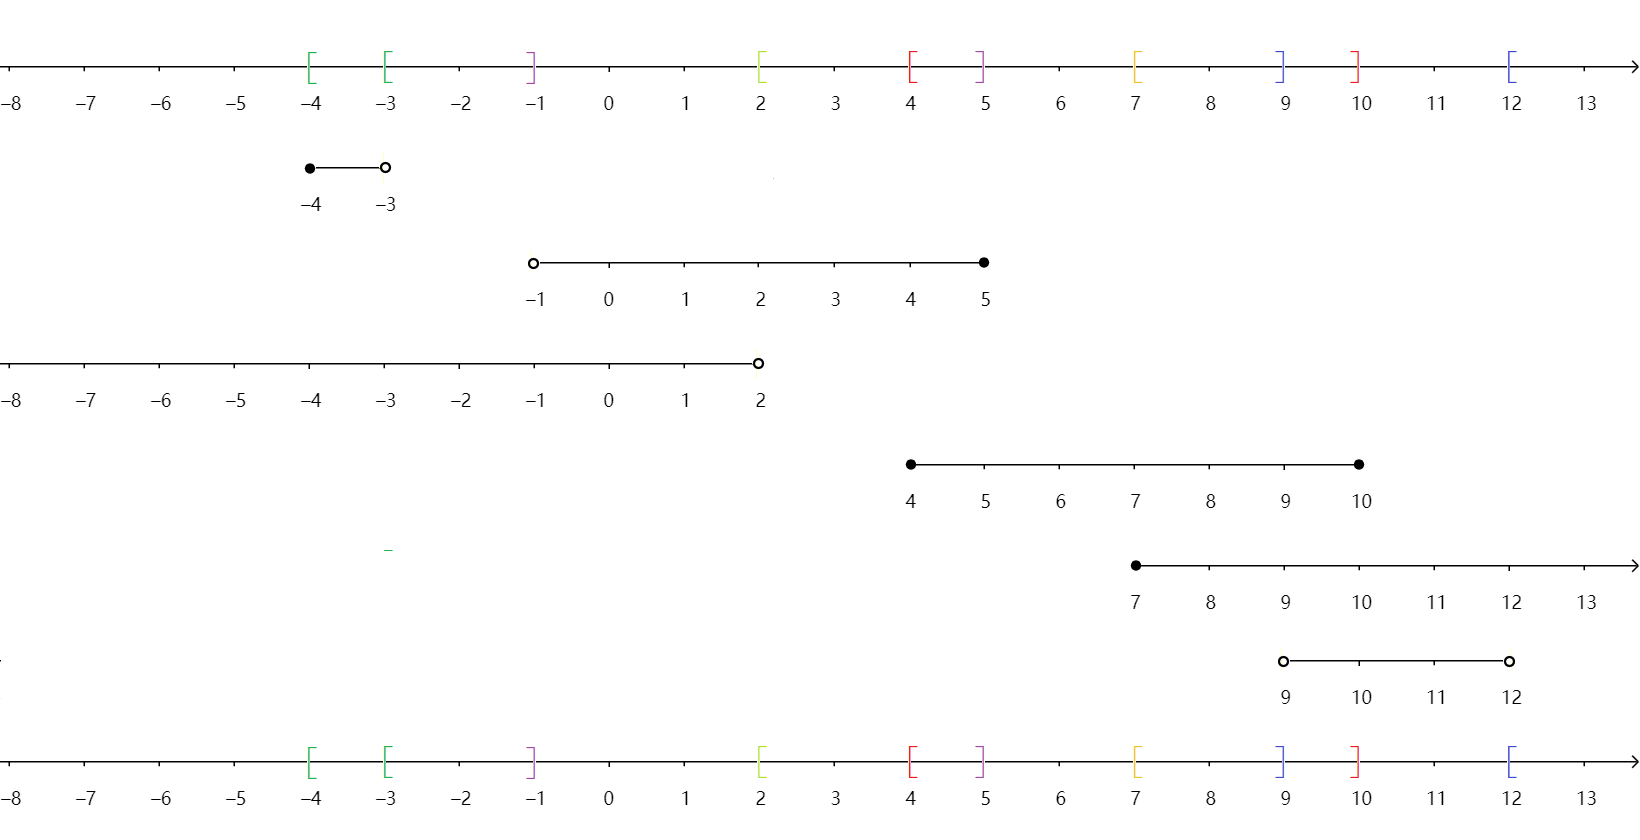
\includegraphics[width=0.96\textwidth]{区间1.png}
\end{figure}

怎么在数轴上表示区间呢?上图展示了两种表示区间的方法。一种是用方括号截断数轴,形成区间。
方括号朝着区间外,说明这一侧是开的(去除端点),否则是闭的(保留端点)。
另一种方法是用实心点和空心点来截断数轴。空心点表示开(去除端点),实心点表示闭(保留端点)。

另外要注意的是,$(a, b)$既可能表示平面上一点的坐标,也可能表示开区间。我们约定,不作特别说明的情况下,
$(a, b)$总表示点的坐标,除非上下文能够表明我们在讨论开区间$(a, b)$。
\begin{sk}\label{sk:5-4-0}
    \mbox{}\\
    \indent 1. 无穷符号和无穷有什么关系?\\
    \indent 2. 能否说:射线和直线是无穷的,线段是有穷的?
\end{sk}
\begin{xt}\label{xt:5-4-0}
    用区间的形式表示以下的集合:\\
    \indent 1. $\{x \, | \, x > -4 \mbox{,而且} x \leqslant 0.4 \}$ \\
    \indent 2. $\{x \, | \, x \geqslant 1 \mbox{且} x \leqslant 5 \mbox{,或者} x < 8  \mbox{且} x > 7.2 \}$ \\
    \indent 3. $\{x \, | \, x \leqslant 3.4 \mbox{,或者} x < 6  \mbox{且} x \geqslant -0.2 \}$
\end{xt}

\section{一元一次不等式组}
来看区间的用途。我们来看这样的问题:
\begin{ex}\label{ex:5-5-0}
    某公司将组装好的轴承件运到海外销售。海运公司运输每船货物的成本是$300$万元。海外铺货等销售成本是$800$万元。
    每箱货物净重导致货船的吃水线升高约$1.3$厘米。货船给某公司留出的余地是$60$厘米。
    估计每箱货物本地销售毛利润是$74$万元,运输过程平均损耗率是$0.6\%$。为使海外销售不亏本,每次运输多少箱货物是可以接受的?
\end{ex}

\begin{so}
    设每次运输$x$箱货物。根据条件,$x$箱货物导致吃水线升高$1.3x$厘米。因此:
    $$ 1.3x \leqslant  60.$$
    此外,$x$箱货物毛利润是$74x$万元。运输过程损耗$0.006x$的货物之后,扣除货运成本和海外销售成本,要使得海外销售不亏本,要有:
    $$ 74 (x - 0.006x) - 300 - 800 \geqslant 0. $$
    以上两个条件必须同时满足,因此问题的解集是以上两个不等式的公共解。
\end{so}

从例子中可以看到,实际生产和生活中,往往需要找到满足多个条件的数。我们把这些条件转化成不等式后,
用大括号括起来,叫做不等式组。从集合的角度来看,我们要找的是多个集合的交集。比如,上题中的两个不等式就可以写成:
$$ \quad \quad \quad \quad \quad\left\{
\begin{array}{cr}
    1.3x \leqslant 60, & \quad \quad \quad \quad \quad (1) \\
    73.556x \geqslant 1100, & \quad \quad \quad \quad \quad (2)
\end{array}\right.
$$
从不等式$(1)$可以解出:$x \leqslant \frac{60}{1.3} \approx 46.154$。从不等式$(2)$可以解出$x \geqslant \frac{1100}{73.556} \approx 14.955$。
所以,$(1)$的解集是区间$(-\infty, \frac{60}{1.3}]$,$(2)$的解集是区间$[\frac{1100}{73.556}, +\infty)$。
它们的交集是:
$$(-\infty, \frac{60}{1.3}] \cap [\frac{1100}{73.556}, +\infty)  = [\frac{1100}{73.556}, \frac{60}{1.3}]. $$
在数轴上画出这两个区间,可以更直观地理解这个步骤。在数轴上看,取两个区间的交集,就是取它们重叠的部分。

\begin{figure}[H] %this figure will be at the right
    \vspace{8pt}
    \centering
    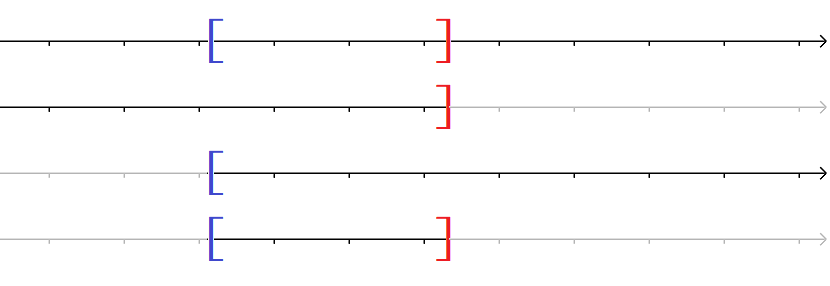
\includegraphics[width=0.6\textwidth]{一元一次不等式组1.png}
\end{figure}

由于箱数必然是整数,我们只考虑区间$[\frac{1100}{73.556}, \frac{60}{1.3}]$中的整数。
因此,问题的解集是:$\{n \, | \, n \in \mathbb{Z} \mbox{ 且 }15 \leqslant n \leqslant 46\}$。
我们一般把这样的整数集合简记为:$[15 \, \ldots \, 46]$。

如果我们想知道每次运输到海外销售,获利和数量的关系是怎样的,
我们可以建立箱数和利润(万元)之间的函数关系:
$$ x \mapsto 74 (x - 0.006x) - 300 - 800 = 73.556 x - 1100. $$
如果我们不考虑亏损的话,这个函数的定义域可以是$[0 \, \ldots \, 46]$。如果不希望亏损,
那么可以把定义域限定在$[15 \, \ldots \, 46]$。

\begin{xt}\label{xt:5-5-0}
    解不等式组:\\
    \indent 1. $\left\{
        \begin{array}{cr}
            1.2x + 8 < 53.9 \\
            3 - 2.6x \leqslant 16 
        \end{array}\right.$ \\
    \indent 2. $\left\{
        \begin{array}{cr}
            2x - 7 < 0 \\
            1 + 1.5x \geqslant 9.5 \\
            -0.2x + 0.6 < 1.2 
        \end{array}\right.$ 
\end{xt}

\chapter{多变量的问题}
我们来看下面的问题:
\begin{quote}
    已知两个数的和是$7$,求这两个数。
\end{quote}
这个问题里有两个未知数。如果设其中一个数是$x$,另一个是$y$,根据题意,
可以列出方程:
$$ x + y = 7.$$
这个方程里有两个变量来表示未知数,并且含有变量的项都是一次项。这样的方程叫做\textbf{二元一次方程}。
二元一次方程是由关于未知数的二元一次式构成的方程。

$x=3, y=4$时,方程成立,因此,$x=3, y=4$是方程的一个解。
$x=2.4, y=4.6$时,方程也成立,因此,$x=2.4, y=4.6$也是方程的一个解。
我们也可以把解写成$(3, 4)$或$ \left\{ \begin{array}{c}
    x = 3, \\
    y = 4.
\end{array}\right.$

如果把方程改写成:$ y = 7 - x.$
那么,$x$取任意数的时候,将$y$对应$7 - x$得到的数,就得到方程的一个解。
比如:
$$
\begin{array}{ll}
    \mbox{取}x = 1\mbox{时,} & \mbox{可以得到 }y = 6\mbox{;} \\
    \mbox{取}x = 2\mbox{时,} & \mbox{可以得到 }y = 5\mbox{;}  \\
    \mbox{取}x = -0.8\mbox{时,} & \mbox{可以得到 }y = 7.8\mbox{;}  \\
    \mbox{取}x = 31\mbox{时,} & \mbox{可以得到 }y = -24\mbox{;等等。} 
\end{array}
$$
如果$x,y$可以取任意实数,那么这个方程的解集是$\{(a, 7-a) \,|\, a \in \mathbb{R}\}$,
它是$\{(a, b) \,|\, a,b\in\mathbb{R}\}$的子集。

\section{二元一次方程组}
实际生活中,包含多变量的问题往往也包含不止一个相等关系。我们来看另一个问题:
\begin{quote}
    甲乙两数和是$7$,且甲比乙大$3$,问甲乙各是多少?
\end{quote}
这个问题包含了两个未知数,也包含了两个相等关系。可以列出两个方程:
$$ \quad \quad \quad \quad \quad\left\{
\begin{array}{cr}
     x + y = 7, & \quad \quad \quad \quad \quad (1) \\
     x - y = 3, & \quad \quad \quad \quad \quad (2)
\end{array}\right.
$$
我们要求$x$和$y$既满足$(1)$,又满足$(2)$。因此,用大括号把这两个方程括起来,求它们的公共解。
这样的多个方程,称为\textbf{方程组}。由几个一元方程组成,关于两个变量的方程组,叫做\textbf{二元一次方程组}。\\
$ \left\{ \begin{array}{c}
    x = 3, \\
    y = 4.
\end{array}\right. ,\quad \left\{ \begin{array}{c}
    x = 5, \\
    y = 2.
\end{array}\right. ,\quad \left\{ \begin{array}{c}
    x = -1, \\
    y = 8.
\end{array}\right.\cdots $都是$(1)$的解;\\
$ \left\{ \begin{array}{c}
    x = 6, \\
    y = 3.
\end{array}\right. ,\quad \left\{ \begin{array}{c}
    x = 5, \\
    y = 2.
\end{array}\right. ,\quad \left\{ \begin{array}{c}
    x = -1.5, \\
    y = -4.5.
\end{array}\right.\cdots $都是$(2)$的解。\\
其中,$\left\{ \begin{array}{c}
    x = 5, \\
    y = 2.
\end{array}\right.$既是$(1)$的解,也是$(2)$的解,因此是两个方程的公共解,或者说\textbf{方程组的解}。
用集合的说法,方程组的解集是各个方程解集的交集。

\section{消元法}
怎么解二元一次方程组呢?我们介绍一种常用的方法:\textbf{消元法}。

消元法的思路是:从二元一次方程组出发,得到一元一次方程,从而求出解。二元一次方程组比一元一次方程多一个元。
因此,要消去一个元。

从上一节的方程组出发:
$$ \quad \quad \quad \quad \quad\left\{
\begin{array}{cr}
     x + y = 7, & \quad \quad \quad \quad \quad (1) \\
     x - y = 3, & \quad \quad \quad \quad \quad (2)
\end{array}\right.
$$
我们把$(1)$改写成$y = 7 - x$,用$x$表示$y$。然后将$(2)$中的$y$用关于$x$的表达式代替,得到一个关于$x$的一元一次方程。:
$$ x - (7 - x) = 3.$$
解这个方程,得$x = 5$。而$y$可以用$x$表示,因此可以求出$y$:$y = 7 - x = 2$。
经过检验,得出方程组的解是:$\left\{ \begin{array}{c}
    x = 5, \\
    y = 2.
\end{array}\right.$

以上方法把从方程组的一个方程出发,把一个变量用另一个变量表示,代入别的方程,消去变量。
这种方法叫做\textbf{代入消元法},简称\textbf{代入法}。它可以概括为:
\begin{center}
    \fbox{
        \shortstack[l]{
            1. 选定一个方程和其中一个系数不为零的变量。\\
            2. 根据等式的基本性质,把这个变量写成另一个变量的表达式。\\
            3. 将它的表达式代入其它的方程,这样这个变量就被消去了,只\\
            $\,\,\,\,\,$剩下关于另一个变量的一元一次方程。\\
            4. 解出另一个变量的值。\\
            5. 将另一个变量的值代入第二步中的表达式,解出消去变量的值。
        }
    }
\end{center}

再看另一种方法。仍然从上一节的方程组出发。观察$(2)$中含$y$的项,系数是$-1$,
而$(1)$中含$y$的项,系数是$1$。将等式$(1)$两边各乘以$1$,然后用$(2)$分边加上它,
就得到:
$$ x - y + 1 \cdot (x + y) = 3 + 1 \cdot 7.$$
注意到$y$的系数为$-1 + 1 \cdot 1 = 0$,含$y$的项被消掉了。只剩下含$x$的项。上式化简得到一元一次方程:
$$ 2x = 10.$$
解这个方程得$x = 5$,代入$(1)$得到$y = 2$。经过检验,得出方程组的解是:$\left\{ \begin{array}{c}
    x = 5, \\
    y = 2.
\end{array}\right.$

以上方法从方程组的一个方程出发,通过在两边乘以适当的系数后和其它方程相加,消去其它方程中的某个变量。
这种方法叫\textbf{增减消元法},简称\textbf{增减法}。它可以概括为:
\begin{center}
    \fbox{
        \shortstack[l]{
            1. 选定一个方程和其中一个系数不为零的变量。\\
            2. 将方程两边乘以适当的数,使得第一步中变量的系数和\\
            $\,\,\,\,\,$另一个方程中的系数是相反数。\\
            3. 把新得到的方程分边和另一个方程相加,这样这个变量就被\\
            $\,\,\,\,\,$消去了。\\
            4. 解出另一个变量的值。\\
            5. 将另一个变量的值代入第一步中的方程,解出消去变量的值。
        }
    }
\end{center}

第二步中,如何选取适当的数呢?我们再来看一个例子。
$$ \quad \quad \quad \quad \quad\left\{
\begin{array}{cr}
     4x + 3y = 7, & \quad \quad \quad \quad \quad (1) \\
     x + 2y = 3, & \quad \quad \quad \quad \quad (2)
\end{array}\right.
$$
我们仍然想消去$y$。选定第一个方程,$y$的系数是$3$。要将方程两边乘以适当的数$a$,让$y$的系数变成$2$的相反数。
因此我们可以列出方程:
$$ 3a = -2.$$
即$a = -\frac{2}{3}$。这样,$(1)$乘以$-\frac23$得到的新方程和$(2)$相加,就得到:
$$ \left(1 + (-\frac{2}{3}) \cdot 4\right) x = 3 + (-\frac{2}{3}) \cdot 7.$$
解得$x = 1$,代入第一个方程得到$y = 1$。经过检验,得出方程组的解是:$\left\{ \begin{array}{c}
    x = 1, \\
    y = 1.
\end{array}\right.$

总结:第二步中,适当的数可以通过解关于变量系数的一元一次方程得到。为了使方程有解,第一步要选系数不为$0$的变量。

\begin{xt}\label{xt:6-1-0}
    解以下方程组:\\
    \indent 1. $ \left\{
        \begin{array}{cr}
             2x - 3y = 2\\
             3x + 2y = 16
        \end{array}\right.
        $ \\
    \indent 2. $\left\{
        \begin{array}{cr}
                7x + y = -2\\
                -4x + 2y = 14
        \end{array}\right.
        $ 
\end{xt}

\section{多元一次方程组举例}
观察以上解答,可以发现,消元法只用到了四则运算。
用消元法的思想,不仅可以解二元一次方程组,也可以解关于更多变量的一次方程组。

我们来看这样一个方程组:
$$ \quad \quad \quad \quad \quad\left\{
\begin{array}{cr}
     x - 3y + z = 2, & \quad \quad \quad \quad \quad (1) \\
     4x - y - z = 9, & \quad \quad \quad \quad \quad (2) \\
     y + 3z = 7, & \quad \quad \quad \quad \quad (3)
\end{array}\right.
$$
用增减法解这个方程组。首先消去$x$。选取$(1)$,两边乘以$-4$后,与$(2)$相加,得到:
$$ \quad\quad\quad\quad\quad 11y -5z = 1.\quad\quad\quad\quad\quad (2')$$
$(3)$中本来就没有$x$,所以$(2')$和$(3)$构成二元一次方程组:
$$ \quad \quad \quad \quad \quad\left\{
\begin{array}{cr}
    11y -5z = 1, & \quad \quad \quad \quad \quad (2') \\
    y + 3z = 7. & \quad \quad \quad \quad \quad (3) 
\end{array}\right.
$$
接下来再消去$y$。选取$(3)$,两边乘以$-11$后,和$(2')$相加,得到一元一次方程:
$$ -38z = -76.$$
解得$z = 2$,代入$(3)$得到$y = 1$;再代入$(1)$得到$x = 3$。经过检验,得出方程组的解是:$\left\{ \begin{array}{c}
    x = 3, \\
    y = 1, \\
    z = 2.
\end{array}\right.$

以上的方程组总有一个解。是不是一次方程组总有解呢?我们来看这样一个方程组:
$$ \quad \quad \quad \quad \quad\left\{
\begin{array}{cr}
     x + 3y = 0, & \quad \quad \quad \quad \quad (1) \\
     -x - 3y = 3, & \quad \quad \quad \quad \quad (2)
\end{array}\right.
$$
用增减法消去$x$,得到:$0 = 3$。这个等式总是不成立的,因此方程组无解。另一方面,如果$(2)$的右边是$0$而不是$3$,
那么用增减法消去$x$,就得到:$0 = 0$。这个等式总是成立的,因此方程有任意解。

\section{图像法}
我们已经了解过如何用图像法解一元一次方程和一元一次不等式。建立直角坐标系后,
一元一次式对应着平面中的直线。一元一次方程的解对应着直线和$x$轴的交点,
而一元一次不等式的解集对应直线在$x$轴上方或下方的部分。

如何在平面中表示二元一次方程组呢?仍然从第一节的方程组出发:
$$ \quad \quad \quad \quad \quad\left\{
\begin{array}{cr}
     x + y = 7, & \quad \quad \quad \quad \quad (1) \\
     x - y = 3, & \quad \quad \quad \quad \quad (2)
\end{array}\right.
$$
我们已经发现,$x$取任意数时,$y$取$7 - x$,就得到$(1)$的一个解。
也就是说,点$(x, y)$是$(1)$的一个解,当且仅当$y = 7 - x$。考虑一次函数:$x \mapsto 7 - x$。
它的图像是一条直线,而且它的图像中每一个点$(x, y)$,就是$(1)$的一个解。
于是我们有这样的结论:
\begin{tm}
    二元一次方程的解集对应平面中一条直线。
\end{tm}
两种特殊情形需要注意:$x$或$y$的系数等于$0$,这时方程的解集分别对应平行于$x$轴和平行于$y$轴的直线。
比如,$y = 7$的解集是$\{(x, 7) \,|\, x\in\mathbb{R}\}$,这是一条平行于$x$轴的直线;
$x = 4$的解集是$\{(4, y) \,|\, y\in\mathbb{R}\}$,这是一条平行于$y$轴的直线。

\begin{wrapfigure}[12]{r}{0.5\textwidth} %this figure will be at the right
    \vspace{-15pt}
    \flushright
    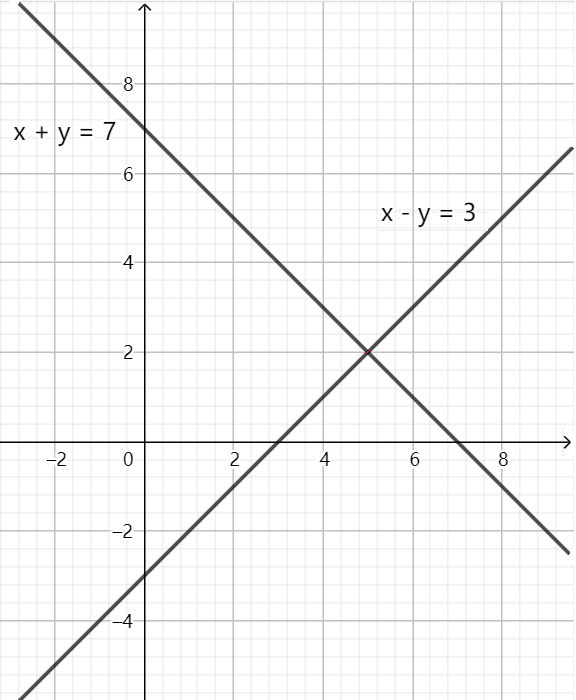
\includegraphics[width=0.48\textwidth]{二元一次方程组.png}
\end{wrapfigure}

二元一次方程组的解集,是它包含的各个二元一次方程解集的交集。所以,以上方程组的解集,
就是$x + y = 7$解集对应的直线和$x - y = 3$解集对应的直线的交点。
在平面直角坐标系中作出这两条直线,它们的交点就是方程组的解。

因为两条直线要么平行,要么相交,要么重合,所以两个方程构成的二元一次方程组
要么无解,要么恰有一个解,要么有任意解。

\begin{sk}\label{sk:6-3-0}
    \mbox{}\\
    \indent 1. 设某个二元一次方程组由$3$个方程组成。它的解集可能有哪些情况?$4$个、$5$个方程组成的方程组呢?\\
    \indent 2. 三元一次方程组能否对应平面中的形状?你有什么想法?
\end{sk}


\end{document}